
%!TEX encoding = IsoLatin 

%%%%%%%%%%%%%%%%%%%%%%%%%%%%%%%%%%%%%%%%%%%%%%%%%%%%%%%%%%%%%%%%%%%%%
%
% %
% 
%%%%%%%%%%%%%%%%%%%%%%%%%%%%%%%%%%%%%%%%%%%%%%%%%%%%%%%%%%%%%%%%%%%%%




\documentclass[12pt,a4paper]{report}

\usepackage{fontspec}
\usepackage{lipsum}

\usepackage{xltxtra}

\setmainfont{Cambria}
%\usefonttheme{serif}
%\usefonttheme{professionalfonts}

\usepackage{pdfpages}

\usepackage{bclogo}
\usepackage{url}

\usepackage{polyglossia} 
\setdefaultlanguage{french}

% marges

\setlength{\topmargin}{-1.54cm}         % marge supÈrieure (retirer 2.54 cm)
\setlength{\oddsidemargin}{-0.04cm}     % marge de gauche (retirer 2.54 cm)
\setlength{\textwidth}{15.3cm}          % largeur du texte
\setlength{\textheight}{21.4cm}         % hauteur du texte
\setlength{\unitlength}{7ex}            % unitÈ pour graphiques

\usepackage{harvard}
%\usepackage[latin1]{inputenc}

%\usepackage[francais]{babel}
\usepackage{amssymb}
%\usepackage[french]{babel}
\usepackage{amsmath}
\usepackage{boxedminipage}
\usepackage{amsthm}
%\usepackage[dvips]{graphicx}
%\usepackage{color}
%\usepackage{epic}
%\graphicspath{{Figures/}} 

\usepackage{pgfplots}
\usepackage{ifpdf}
\usepgfplotslibrary{groupplots}
\usetikzlibrary{backgrounds}
\ifpdf\else
  \usepackage{pstricks,pst-node,pst-plot,pst-circ}
  \psset{pgffunctions}
\fi
\pgfplotsset{width=7cm,compat=1.6}

\usepackage{tikz}
\usepackage{tikz-3dplot}
\usepackage{float}





%\usepackage{hyperref}

\theoremstyle{plain} %\part{title}
\theoremstyle{definition}
\newtheorem{definition}{Définition}[section]
\newtheorem{example}{Exemple}[section]
\newtheorem{theorem}{Théorême}[section]
\newtheorem{lemma}{Lemme}[section]
\newtheorem{proposition}{Proposition}[section]
\newtheorem{corollary}{Corollaire}[section]

\theoremstyle{remark}
\newtheorem*{conjecture}{\indent Conjecture}
\newtheorem*{remark}{\indent Remarque}



\newcommand{\N}{\mathbb{N}}                     
\newcommand{\R}{\mathbb{R}}      
\newcommand{\C}{\mathbb{C}}
\newcommand{\Z}{\mathbb{Z}}
\newcommand{\K}{\mathbb{K}} 
\newcommand{\LL}{\mathcal{L}}                 
\newcommand{\M}{\mathcal{M}}    



\renewcommand{\labelitemi}{$\bullet$}

%%%%%%%%%%%%%%%%%%%%%%%%%%%%%%%%%%%%%%%%%%%%%%%%%%%%%%%%%%%%%%%%%%%%%
%\hypersetup{
%backref=true, %permet d'ajouter des liens dans... %pagebackref=true,%...les bibliographies
%hyperindex=true, %ajoute des liens dans les index.
%colorlinks=true, %colorise les liens
%breaklinks=true, %permet le retour a? la ligne dans les liens trop longs urlcolor= blue, %couleur des hyperliens
%linkcolor= blue, %couleur des liens internes
%bookmarks=true, %cre?e? des signets pour Acrobat
%}

\parskip 7pt

%\parindent 0pt

\newcommand{\inttotal}{\int_{-\infty}^{\infty}}
\newcommand{\intpositive}{\int_{0}^{\infty}}
\newcommand{\om}{\omega}
\newcommand{\BF}{{\cal F}} 

\newcounter{numeroexo}
\newcommand{\exercice}{\par\noindent\stepcounter{numeroexo}
        \hspace{-.25cm}\fbox{\textbf{Exercice \arabic{numeroexo}}}\quad}



%%%%%%%%%%%%%%%%%%%%%%%%%%%%%%%%%%%%%%%%%%%%%%%%%%%%%%%%%%%%%%%%%%%%%

% Pour ne compiler qu'un chapitre :
%\includeonly{transfo_fourier}

\begin{document}

\begin{titlepage}

\includegraphics[width=5cm]{logo-polytech.pdf}

\vfill 
{\huge Analyse de Fourier} \\

{\huge INFO 3} \\

\vfill

%{\Large M. Gelgon et al.  \footnote{Nombreuses contributions de Jp Guédon, V.Ricordel, J.Cohen, N.Normand} \\
%Département informatique \\
%Ecole polytechnique de l'université de Nantes}  \\

%Ce document sert de support d'enseignement pour un cours-TD de 12h, pour un public d'élèves-ingénieurs en informatique (1ere année de cycle ingénieur). Dans le cursus ingénieur, il est suivi par des enseignements sur traitement du signal discret et sur les données multimédia, où les concepts vus ici sont prolongés et illustrés.  Ce cours est aussi une occasion de voir ou revoir, en les manipulant dans le contexte de l'analyse de Fourier, des concepts mathématiques classiques pour le calcul d'intégrales, les espaces de fonctions.

\vfill
CC-BY-NC-SA  \\

M. Gelgon, N. Normand, V. Ricordel \\

Point de contact pour remarques et corrections : marc.gelgon@univ-nantes.fr

Dernière compilation : \today


\end{titlepage}

\tableofcontents
%\listoffigures
%\bibliographystyle{agsm}
%\bibliography{biblio}

%%%%%%%%%%%%%%%%%%%%%%%%%%%%%%%%%%%%%%%%%%%%%%%%%%%%%%%%%%%%%%%%%%%%%
%\pagebreak


\chapter{Intuitions sur les espaces de fonctions}

Ce cours se veut volontairement informel sur nombre de points mathématiques. Il passe sous silence de nombreuses hypothèses et ne formalise pas les espaces de fonctions \footnote{\url{https://fr.wikipedia.org/wiki/Espace_fonctionnel}} ni les distributions \footnote{\url{https://fr.wikipedia.org/wiki/Distribution_(mathématiques)}}, par exemple, alors qu'il les manipule. Quand on passe à la mise en oeuvre informatique (numérique et discrétisée) des concepts traités dans ce cours, beaucoup de ces difficultés ne se posent néanmoins plus.

\section{Composition-décomposition de vecteurs dans \texorpdfstring{$\RR^n$}{\pdfRR\superscriptn}}

\subsection{L'espace vectoriel \texorpdfstring{$\RR^n$}{\pdfRR\superscriptn}, décomposition dans la base canonique}

On a l'habitude de se représenter de façon géométrique des vecteurs dans $\RR^n$ et de les manipuler (par exemple, les ajouter). En particulier, considérant $\RR^n$ comme un espace vectoriel et disposant d'une base $(e_1,....,e_n)$ dans cet espace (la base canonique ou une autre), l'algèbre linéaire établit qu'on peut fabriquer n'importe quel vecteur $u$ de $\RR^n$ en construisant une combinaison linéaire des vecteurs de cette base (ici les $a_i$ sont des réels):
\begin{equation}
u=a_1.e_1+\dots+a_n.e_n
\label{eq:decomposition_lineaire}
\end{equation} 
Il est également établi que cette combinaison linéaire est unique, c.a.d. qu'étant donné un vecteur $u$ et une base $(e_1,....,e_n)$, il existe un et un seul ensemble de coefficients $(a_1,....,a_n)$ tel que $u=a_1.e_1+\dots+a_n.e_n$.

\subsection{Décomposition d'un vecteur dans une base quelconque}

\subsubsection{Par résolution d'un sytème linéaire}

Etant donné un vecteur $u$ dans $\RR^n$, on peut avoir besoin de récupérer les coefficients $a_i$ de la décomposition de $u$ dans une base donnée.
 S'il s'agit de la base canonique, ces coefficients sont simplement les composantes du vecteur. S'il s'agit d'une autre base, cela peut, par exemple, se faire en résolvant un système de $n$ équations à $n$ inconnues (qui sont les $a_i$).

Par exemple, soit le vecteur $u=(5,3)^T$. Il se décompose sur la base canonique comme  
\begin{equation}
\begin{pmatrix} 5 \\ 3 \end{pmatrix} = 5  \begin{pmatrix} 1 \\ 0 \end{pmatrix} + 3  \begin{pmatrix} 0 \\ 1 \end{pmatrix}
\end{equation}
On peut identifier $a_1=5$ et $a_2=3$ immédiatement.

Si on souhaite décomposer $u$ sur une autre base, par exemple la base formée par les vecteurs $e_1=(1,1)^T$ et $e_2=(-1,1)^T$, pour identifier $a_1$ et $a_2$, il faut résoudre
\begin{equation}
\begin{pmatrix} 5 \\ 3 \end{pmatrix}  = a_1  \begin{pmatrix} 1 \\ 1 \end{pmatrix} + a_2  \begin{pmatrix} -1 \\ 1 \end{pmatrix}
\end{equation}
En écrivant cette équation comme 2 équations à 2 inconnues, on trouve rapidement $a_1=4$ et $a_2=-1$.

\subsubsection{Par projections orthogonales}

Regardons maintenant comment on peut obtenir les coefficients de la décomposition d'un vecteur $u$ sur une base de $\RR^n$, en utilisant des projections orthogonales. 

$\RR^n$ est un espace vectoriel, ce qui permet de faire des combinaisons linéaires de vecteurs, comme ci-dessus. Pour faire des projections orthogonales, il faut enrichir notre espace vectoriel avec un opérateur: le \textbf{produit scalaire}. Dans $\RR^n$, notons $\langle u , v \rangle$ le produit scalaire entre deux vecteurs $u=(u_1,\dots,u_n)$ et $v=(v_1,\dots,v_n)$. La définition simple du produit scalaire dans $\RR^n$ est : 
\begin{equation}
\langle u , v \rangle = \sum_{i=1}^n u_i.v_i
\end{equation}
La \textbf{norme euclidienne} $\|u\|$ d'un vecteur $u=(u_1,\dots,u_n)$ de $\RR^n$, qui décrit intuitivement sa longueur indépendamment de son orientation, est définie à partir du produit scalaire $\langle u, u \rangle$ comme 
\begin{equation}
\|u\|= \sqrt{\langle u, u \rangle}=\sqrt{\sum_i u_i^2}
\end{equation}

Le produit scalaire entre deux vecteurs $u$ et $v$ de $\RR^n$, tels qu'il y a un angle $\theta$ entre $u$ et $v$, peut se calculer comme:
\begin{equation}
\langle u, v \rangle=\|u\|.\|v\|cos(\theta)
\end{equation}
Autrement dit, l'\textbf{angle}, du moins ce que peut en déterminer son cosinus, est calculable comme le produit scalaire normalisé par la longueur des vecteurs impliqués dans ce produit scalaire :
\begin{equation}
cos(\theta) = \frac{\langle u, v \rangle}{\|u\|.\|v\|}
\end{equation}

Le produit scalaire permet aussi d'introduire la notion de \textbf{projection orthogonale} d'un vecteur de $\RR^n$ sur un autre. De façon générale, la projection orthogonale d'un vecteur $u$ sur un vecteur $v$ consiste à décomposer $u$ comme la somme d'un vecteur $u$ colinéaire à $v$, noté $u_{\| v}$ (dite "projection orthogonale de $u$ sur $v$") et une partie orthogonale à $v$, notée $u_{\perp v}$. Cette décomposition est unique (on n'en fait pas la démonstration ici).

%La projection d'un vecteur $u$ quelconque sur un vecteur $e_1$ de la base permet de récupérer directement le coefficient $a_1$ associé. 

Appliquons la projection orthogonale au cas où on projete $u$ sur chacun des vecteurs $e_i$ de la base, tour à tour. Prenons ci-dessous le cas de la projection sur $e_1$, le premier vecteur de la base. On s'intéresse à la décomposition de $u$ comme la somme d'un vecteur colinéaire à $e_1$ (dit "projection orthogonale de $u$ sur $e_1$"), noté $u_{\| e_1}$ et d'un vecteur orthogonal à $e_1$, notée $u_{\perp e_1}$.

\begin{equation}
u = \underbrace{\quad u_{\| e_1} \quad}_{\text{projection orthogonale de $u$ sur $e_1$}} + \underbrace{\quad u_{\perp e_1}}_{\text{composante orthogonale à $e_1$ }} \quad
\end{equation}

\begin{center} 
\begin{tikzpicture} [scale=3, axis/.style={->,blue,thick}, vector/.style={-stealth,red,very thick}, 
vector guide/.style={->,dashed,red,thick}]

%standard tikz coordinate definition using x, y, z coords


%tikz-3dplot coordinate definition using x, y, z coords

\pgfmathsetmacro{\ax}{0.8}
\pgfmathsetmacro{\ay}{0.8}
\pgfmathsetmacro{\az}{0.8}

\coordinate (O) at (0,0,0);
\coordinate (P) at (1,0,0);
\coordinate (Q) at (3,1,0);
\coordinate (M) at (3,0,0);
\coordinate (N) at (3,0.74*\ay,0.5*\az);

\draw[axis]   (O) -- (P) node[anchor=north east]{$e_1$};
\draw[vector] (O) -- (Q) node[anchor=south]{$u$}; ; 
\draw[vector guide] (M) -- (Q) node[anchor=north west]{$u_{\perp e_1}$};
%\draw[vector guide]  (P) -- (M);
\draw[vector guide]         (O) -- (M) node[anchor= north east]{$u_{\|e_1}$};

\end{tikzpicture}
\end{center} 

Dans le triangle rectangle, on a :

\begin{equation}
\langle u , e_1 \rangle   = \|u\|.\|e_1\|cos(\widehat{u,e_1})  =  \|u_{\|e_1}\|.\|e_1\| = \langle u_{\|e_1},e_1 \rangle
\end{equation}


Cela nous permet de caractériser la longueur du vecteur $u_{\|e_1}$ : 

\begin{equation}
\|u_{\|e_1}\|  = \frac{\langle u , e_1 \rangle}{\|e_1\|}
\end{equation}

Par ailleurs, comme $u$ et $e_1$ sont colinéaires, on a 
\begin{equation}
u_{\|e_1} = \|u_{\|e_1}\| . \frac{e_1}{\|e_1\|}
\end{equation}

Si bien qu'en conclusion, on peut exprimer $u_{\|e_1}$ en fonction de $e_1$ et identifier le coefficient $a_1$.
\begin{equation}
u_{\|e_1} = \frac{\langle u , e_1 \rangle}{\|e_1\|^2} \quad e_1
\end{equation}

Si les $e_i$ sont orthogonaux deux à deux, c.a.d. qu'on a une \textbf{base orthogonale}, alors on a plus généralement :
\begin{equation}
u = \frac{\langle u , e_1 \rangle}{\|e_1\|^2} \quad e_1 +\dots + \frac{\langle u , e_n \rangle}{\|e_n\|^2} \quad e_n 
\end{equation}
qui est une nouvelle manière d'écrire l'équation (\ref{eq:decomposition_lineaire}) qui donne un moyen de calcul direct des coefficients $a_i$ de la décomposition, grâce au produit scalaire.

Appliquons cela à l'exemple vu plus haut $u=(5,3)^T$ à décomposer sur la base $e_1=(1,1)^T$ et $e_2=(-1,1)^T$ , et on retrouve bien les résultats qu'on avait obtenus par résolution du système linéaire :
\begin{equation*}
a_1=\frac{\langle u , e_1 \rangle}{\|e_1\|^2} = \frac{\langle\begin{pmatrix} 5 \\ 3 \end{pmatrix},\begin{pmatrix} 1 \\ 1 \end{pmatrix}\rangle}{\sqrt{1^2+1^2}^2}=4 \quad \text{et} \quad a_2=\frac{\langle u , e_2 \rangle}{\|e_2\|^2} = \frac{\langle\begin{pmatrix} 5 \\ 3 \end{pmatrix},\begin{pmatrix} -1 \\ 1 \end{pmatrix}\rangle}{\sqrt{(-1)^2+1^2}^2}=-1 
\end{equation*}

Si, de plus, on considère le cas particulier où $\|e_i\|=1$ pour tout $i \in \{1,...,n\}$ (c.a.d. la base est \textbf{orthonormée} en plus d'être orthogonale), alors c'est encore plus simple :
\begin{equation}
u = \langle u , e_1 \rangle ~e_1 +\dots + \langle u , e_n \rangle ~e_n 
\end{equation}

\section{Mêmes notions, mais sur des fonctions}

La raison de tous les rappels ci-dessus est que l'analyse de Fourier travaille sur des concepts analogues, sinon que les éléments de l'espace sont des fonctions au lieu d'être des vecteurs de $\RR^n$. Par exemple, la figure ~\ref{fonctions_orthogonales} illustre comment la combinaison linéaire de quelques fonctions élémentaires (ici trinométriques) permettrait de générer des fonctions très diverses.

%\tdplotsetmaincoords{60}{120} 

\begin{figure}[H]
\begin{center}
\begin{tikzpicture} [scale=3, axis/.style={->,blue,thick}, vector/.style={-stealth,red,very thick}, 
vector guide/.style={dashed,red,thick}]

%standard tikz coordinate definition using x, y, z coords
\coordinate (O) at (0,0,0);

%tikz-3dplot coordinate definition using x, y, z coords

\pgfmathsetmacro{\ax}{0.8}
\pgfmathsetmacro{\ay}{0.8}
\pgfmathsetmacro{\az}{0.8}

\coordinate (P) at (\ax,\ay,\az);

%draw axes
\draw[axis] (0,0,0) -- (1,0,0) node[anchor=north east]{$sin(x)$};
\draw[axis] (0,0,0) -- (0,1,0) node[anchor=north east]{$sin(2x)$};
\draw[axis] (0,0,0) -- (0,0,1) node[anchor=east]{$cos(x)$};

%draw a vector from O to P
\draw[vector] (0,0,0) -- (1,2,1) node[anchor=south]{$cos(x)+sin(x)+2sin(2x)$}; ; 

%draw guide lines to components
%\draw[vector guide]         (O) -- (\ax,\ay,0);
%\draw[vector guide] (\ax,\ay,0) -- (P);
%\draw[vector guide]         (P) -- (0,0,\az);
\draw[vector guide] (1,2,1) -- (0,0,1);
\draw[vector guide] (1,2,1) -- (1,0,0);
\draw[vector guide] (1,2,1) -- (0,2,0);
\draw[vector guide] (0,0,0) -- (0,2,0);
%\node[tdplot_main_coords,anchor=east]
%at (\ax,0,0){(\ax, 0, 0)};
%\node[tdplot_main_coords,anchor=west]
%at (0,\ay,0){(0, \ay, 0)};
%\node[tdplot_main_coords,anchor=south]
%at (\ax,0:ay,\az){(0, 0, \az)};
\end{tikzpicture}
\begin{tikzpicture}
\begin{axis}[scale=0.63,xlabel={x (en degrés)},title={cos(x)+sin(x)+2sin(2x) (en gras) }]
 \addplot[domain=0:360, samples= 100, blue,  ultra thick]{cos(x)+sin(x)+2*sin(2*x)};
 \addplot[domain=0:360, samples= 100, blue]{cos(x)};
 \addplot[domain=0:360, samples= 100, blue]{sin(x)};
 \addplot[domain=0:360, samples= 100, blue]{sin(2*x)};
\end{axis}
\end{tikzpicture}
\end{center}
\caption{Représentation intuitive d'un espace de fonctions. Par exemple, la famille $(cos(x),sin(x),sin(2x))$ permet de générer une infinité de fonction par combinaison linéaire $a_1.cos(x)+a_2.sin(x)+a_3.sin(2x)$ où les $a_i \in \RR$. Par exemple, l'illustration correspond au cas (arbitraire) $a_1=1,a_2=1,a_3=2$.} Les courbes en trait fin sont cos(x), sin(x) et sin(2x).
\label{fonctions_orthogonales}
\end{figure}

Il reste utile de garder à l'esprit les interprétations géométriques qu'on a pour les vecteurs. On précise maintenant des adaptations des définitions et interprétations dans le cas des fonctions :

\subsection{Produit scalaire entre fonctions}
\label{sec:prodscal}

Soit l'espace $E$ sur $\RR$ des fonctions continues sur
$[a,b]$ vers $\RR$. Définissons un\footnote{``un'' et non ``le'' car
on pourrait en définir d'autres, mais celui-ci est de loin le plus usuel.} produit scalaire entre deux fonctions $f$ et $g$ de cet espace :
\begin{eqnarray}
E \times E & \rightarrow & \RR \nonumber \\
\langle f, g \rangle & \mapsto & \int_a^b f(x)\; g(x)\; dx
\end{eqnarray}

Le premier point à remarquer est que cette définition est semblable à cette qu'on a pour un produit scalaire usuel entre vecteurs : on fait la somme des produits sur les composantes du vecteurs - à ceci près que pour les fonctions cette somme est définie sur un espace continu  $[a,b]$ plutôt qu'un ensemble discret de composantes.

L'\textbf{orthogonalité} entre $f$ et $g$ correspond, comme dans $\RR^n$,
au cas où le produit scalaire s'annule :
\begin{equation}
\int_a^b f(x)g(x)=0
\end{equation}


La figure~\ref{premier_exemple} illustre trois exemples simples avec des fonctions orthogonales $f$ et $g$ définies sur $[-3,3]$. Sur ces exemples, les fonctions sont constantes par morceaux pour la commodité du calcul mental, mais de façon générale elles n'ont pas besoin d'être constantes par morceaux.

\begin{figure}
\begin{center}
\begin{tikzpicture}[background rectangle/.style={fill=olive!5}, show background rectangle]
\begin{groupplot}[group style={group size=1 by 3, horizontal sep=2cm, vertical sep=2cm}, xmax=3,ymin=-2,ymax=2,scale=0.6,axis lines=center,xtick distance=1]
\nextgroupplot[title={\textbf{$f(x)$}}]
  \addplot[domain=-3:0, blue, ultra thick] (x,1);
  \addplot[domain=0:3, blue,  ultra thick] (x,0);
\nextgroupplot[title={\textbf{$g(x)$}}]
  \addplot[domain=-3:0, blue, ultra thick] (x,0);
  \addplot[domain=0:3, blue,  ultra thick] (x,1);
\nextgroupplot[title={\textbf{$f(x)g(x)$}}]
  \addplot[domain=-3:0, blue, ultra thick] (x,0);
  \addplot[domain=0:3, blue,  ultra thick] (x,0);
\end{groupplot}
\end{tikzpicture}
\hfill 
\begin{tikzpicture}[background rectangle/.style={fill=olive!5}, show background rectangle]
\begin{groupplot}[group style={group size=1 by 3, horizontal sep=2cm, vertical sep=2cm}, xmax=3,ymin=-2,ymax=2,scale=0.6,axis lines=center,xtick distance=1]
\nextgroupplot[title={\textbf{$f(x)$}}]
  \addplot[domain=-3:0, blue, ultra thick] (x,1);
  \addplot[domain=0:3, blue,  ultra thick] (x,1);
\nextgroupplot[title={\textbf{$g(x)$}}]
  \addplot[domain=-3:0, blue, ultra thick] (x,-1);
  \addplot[domain=0:3, blue,  ultra thick] (x,1);
\nextgroupplot[title={\textbf{$f(x)g(x)$}}]
  \addplot[domain=-3:0, blue, ultra thick] (x,-1);
  \addplot[domain=0:3, blue, ultra thick] (x,1);
\end{groupplot}
\end{tikzpicture}
\hfill 
\begin{tikzpicture}[background rectangle/.style={fill=olive!5}, show background rectangle]
\begin{groupplot}[group style={group size=1 by 3, horizontal sep=2cm, vertical sep=2cm
}, xmax=3,ymin=-2,ymax=2,scale=0.6,axis lines=center,xtick distance=1]
\nextgroupplot[title={\textbf{$f(x)$}}]
  \addplot[domain=-3:0, blue, ultra thick] (x,1);
  \addplot[domain=0:3, blue,  ultra thick] (x,-1);
\nextgroupplot[title={\textbf{$g(x)$}}]
  \addplot[domain=-3:-1.5, blue,  ultra thick] (x,1);
  \addplot[domain=-1.5:0, blue, ultra thick] (x,-1);
  \addplot[domain=0:3, blue,  ultra thick] (x,1);
\nextgroupplot[title={\textbf{$f(x)g(x)$}}]
  \addplot[domain=-3:-1.5, blue, ultra thick] (x,1);
  \addplot[domain=-1.5:0, blue, ultra thick] (x,-1);
  \addplot[domain=0:3, blue, ultra thick] (x,-1);
\end{groupplot}
\end{tikzpicture}
\end{center}
\caption{Les trois colonnes correspondent à trois exemples. Dans les deux premiers cas, l'intégrale entre -3 et 3 du produit des fonctions est nulle, donc les fonctions sont orthogonales. Dans le troisième cas, le produit scalaire vaut -3.}
\label{premier_exemple}
\end{figure}

La définition plus générale du produit scalaire, qui englobe les cas particuliers des vecteurs dans $\RR^n$ et des fonctions, et qu'on pourrait appliquer à encore d'autres types d'objets mathématiques (matrices, ...) est qu'un produit scalaire doit vérifier les propriétés suivantes :

\begin{enumerate}
\item il s'agit d'une \emph{forme linéaire}, i.e. une application
  linéaire dont l'image $\in \RR$ (qui est le corps sur lequel est
  construit l'espace vectoriel dont proviennent $f$ et $g$),
\item cette forme est \emph{bilinéaire} et \emph{symétrique}
  (bilinéaire : linéaire vis-à-vis de $f$ et de $g$),
\item on dit que le produit scalaire est \emph{défini positif},
  c'est-à-dire :
\begin{enumerate}
\item $\forall f \in E, \langle f, f \rangle=\int_a^bf(x)^2 dx~\geq 0 $ 
\item $\langle f, f \rangle=\int_a^bf(x)^2 dx=0 \Longleftrightarrow f=0$
\end{enumerate}
\end{enumerate}
``Produit scalaire'' est donc une expression raccourcie de ``forme
bilinéaire symétrique définie positive''. 

La figure~\ref{exemples_produitscalaire} montre d'autres exemples.

\begin{figure}
\begin{center}
\begin{tikzpicture}[background rectangle/.style={fill=olive!5}, show background rectangle]
\begin{groupplot}[group style={group size=1 by 3},scale=0.55,domain=0:360, axis lines=center]
\nextgroupplot[title={\textbf{$f(x)=sin(x)$}}]
  \addplot[blue, ultra thick] {sin(x)};
\nextgroupplot[title={$g(x)=sin(x)$}]
  \addplot[blue, ultra thick] {sin(x)};
\nextgroupplot[title=$f(x).g(x)$]
  \addplot[cyan,fill,opacity=0.2,ultra thick] {sin(x)*sin(x)};
\end{groupplot}

\node[align=center,font=\bfseries, yshift=2em] (title) 
    at (current bounding box.north)
    {Exemple 1};

\end{tikzpicture}
\begin{tikzpicture}[background rectangle/.style={fill=olive!5}, show background rectangle]
\begin{groupplot}[group style={group size=1 by 3,horizontal sep=2cm, vertical sep=2cm}, scale=0.5,domain=0:360, axis lines=center]
\nextgroupplot[title={$f(x)=sin(x)$}]
  \addplot[blue, ultra thick] {sin(x)};
\nextgroupplot[title={$g(x)=cos(x)$}]
  \addplot[blue, ultra thick] {cos(x)};
\nextgroupplot[title=$f(x).g(x)$]
  \addplot[cyan,fill,opacity=0.13,ultra thick] {sin(x)*cos(x)};
\end{groupplot}
\node[align=center,font=\bfseries, yshift=2em] (title) 
    at (current bounding box.north)
    {Exemple 2};
\end{tikzpicture}
\begin{tikzpicture}[background rectangle/.style={fill=olive!5}, show background rectangle]
\begin{groupplot}[group style={group size=1 by 3,horizontal sep=2cm, vertical sep=2cm}, scale=0.5,domain=0:360, axis lines=center]
\nextgroupplot[title={$f(x)=sin(x)$}]
  \addplot[blue, ultra thick] {sin(x)};
\nextgroupplot[title={$g(x)=sin(2x)$}]
  \addplot[blue, ultra thick] {sin(2*x)};
\nextgroupplot[title=$f(x).g(x)$]
  \addplot[fill=cyan,opacity=0.13,text opacity=1] {sin(x)*sin(2*x)};
\end{groupplot}
\node[align=center,font=\bfseries, yshift=2em] (title) 
    at (current bounding box.north)
    {Exemple 3};
\end{tikzpicture}
\end{center}
\caption{La figure montre trois exemples (les trois colonnes) de produits scalaires entre fonctions. Les abscisses sont en degrés. Le résultat du produit scalaire est l'aire de la zone hachurée dans la 3eme rangée. Attention, ces aires sont à considérer avec leurs signes positif/négatif, c.a.d. que dans l'exemple 1 l'aire totale est positive tandis que dans les exemples 2 et 3 l'aire totale est nulle. Le premier cas est à rapprocher du calcul de la norme d'une fonction (qui elle-même ressemble au calcul de la norme d'un vecteur), tandis que les exemples 2 et 3 illustrent des cas d'orthogonalité, exemples les plus simples qu'on verra généralisables aux fonctions de base des séries de Fourier.}
\label{exemples_produitscalaire}
\end{figure}

\begin{figure}
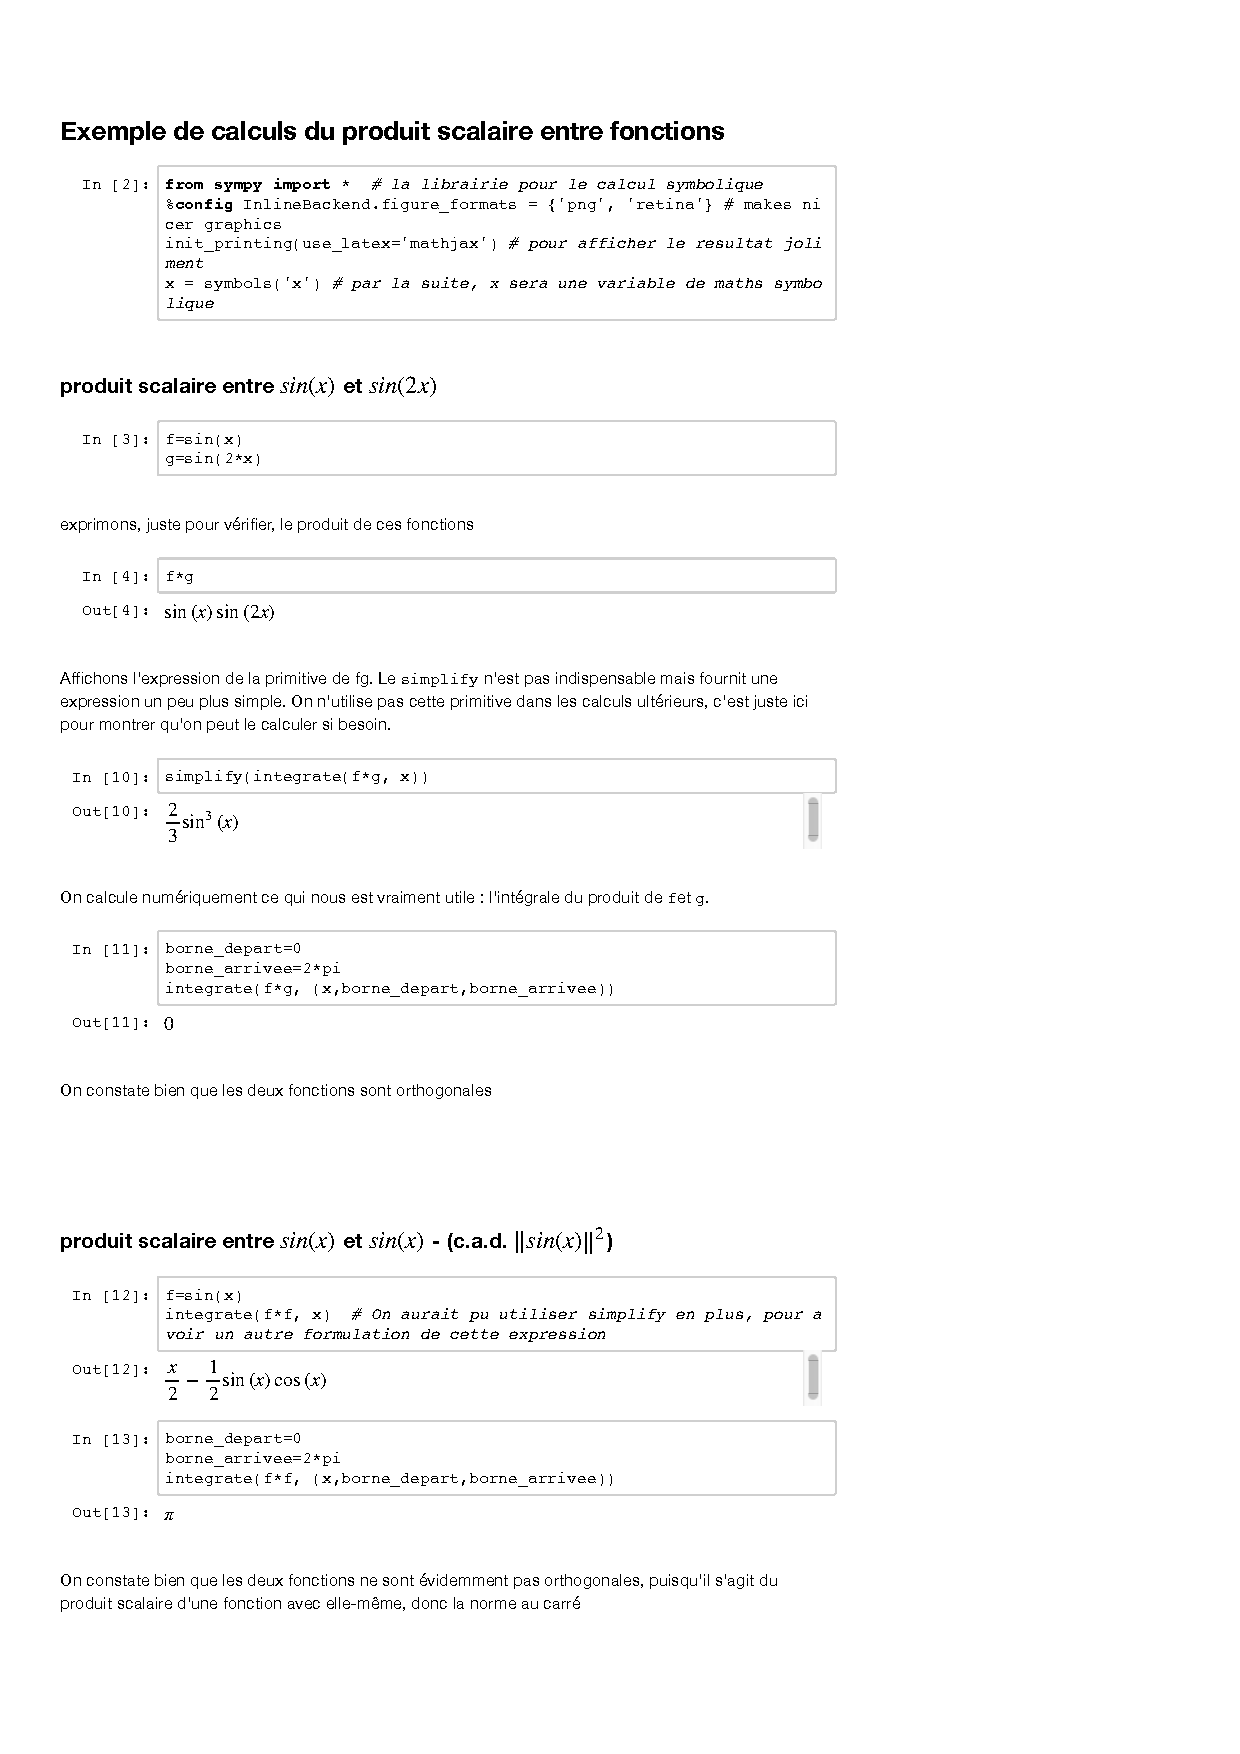
\includegraphics[scale=0.7]{fourier-notebook-polytech.pdf}
\caption{Exemple de calcul symbolique en python pour le calcul d'un produit scalaire entre fonctions.}
\end{figure}

\subsection{Norme d'une fonction}


De façon analogue aux vecteurs, on peut définir la norme (dite \emph{euclidienne}) d'une fonction $f$:
\begin{equation}
\|f\|= \sqrt{\langle f, f \rangle}=\sqrt{\int_a^b f(t)^2dt}
\end{equation} 

\subsection{Angle entre fonctions}


Une définition analogue aux vecteurs peut être construite pour l'angle entre deux fonctions $f$ et $g$:

\begin{equation}
cos(\theta) = \frac{\langle f, g \rangle}{\|f\|.\|g\|}
\end{equation}

%Soient trois vecteurs $v$, $u_1$ et $u_2$ dans $\RR^n$. On s'intéresse à la décomposition suivante :
%
%\begin{equation}
%v = \underbrace{\quad v_{\| u} \quad}_{\text{projection orthogonale de $u_1$ sur $v$}} + \underbrace{\quad v_{\perp u}}_{\text{composante orthogonale à $u$ }} \quad
%\end{equation}
%
%
%
%\begin{center} 
%\begin{tikzpicture} [scale=5, tdplot_main_coords, axis/.style={->,blue,thick}, 
%vector/.style={-stealth,red,very thick}, 
%vector guide/.style={dashed,red,thick}]
%
%%standard tikz coordinate definition using x, y, z coords
%\coordinate (O) at (0,0,0);
%
%%tikz-3dplot coordinate definition using x, y, z coords
%
%\pgfmathsetmacro{\ax}{0.8}
%\pgfmathsetmacro{\ay}{0.8}
%\pgfmathsetmacro{\az}{0.8}
%
%\coordinate (P) at (0.8*\ax,1*\ay,2*\az);
%
%%draw axes
%\draw[axis] (0,0,0) -- (1,0,0) node[anchor=north east]{$u_1$};
%\draw[axis] (0,0,0) -- (0,1,0) node[anchor=north west]{$u_2$};
%%\draw[axis] (0,0,0) -- (0,0,1.5) node[anchor=east]{};
%
%%draw a vector from O to P
%\draw[vector] (O) -- (P) node[anchor=south]{$v$}; ; 
%
%%draw guide lines to components
%
%\coordinate (M) at (0,0.74*\ay,0);
%\coordinate (N) at (0,0.74*\ay,0.5*\az);
%\coordinate (Q) at (0.5*\ax,0,0);
%\coordinate (R) at (0.5*\ax,0.74*\ay,0);
%\coordinate (S) at (0.0*\ax,0.0*\ay,0.9*\az);
%
%\draw[vector guide]         (N) -- (N) node[anchor=north west]{$v_{\perp u_2}$};
%
%\draw[vector guide]         (P) -- (M);
%\draw[axis]         (O) -- (M) node[anchor=north east]{$v_{\|u_2}$};
%\draw[axis]         (O) -- (Q) node[anchor=west]{$v_{\|u_1}$};
%\draw[axis]         (O) -- (R) node[anchor=north east]{$v_{\|u_1}+v_{\|u_2}$};
%\draw[vector guide]         (P) -- (Q); 
%\draw[vector guide]         (S) -- (S) node[anchor=south]{$v_{\perp u_1}$};
%\draw[vector guide]         (P) -- (R) node[anchor=north east]{$v_{\perp u_{1,2}}$};
%
%\end{tikzpicture}
%\end{center} 
%Caractérisons la longueur du vecteur $v_{\|u}$ : 
%
%\begin{equation}
%\langle u , v \rangle   = \langle u , v_{\|u} \rangle
%\end{equation}
%
%\begin{equation}
%\|u\|.\|v\|cos(\widehat{u,v})  =  \|u\|.\|v_{\|u}\|
%\end{equation}
%
%\begin{equation}
%\|v_{\|u}\|  = \frac{\langle u , v \rangle}{\|u\|}
%\end{equation}
%
%Le cas d'utilisation qui nous intéresse principalement ici est celui où $v$ est un vecteur quelconque et $u$ un vecteur de base (généralement parmi d'autres vecteurs de base), dont nous souhaitons déterminer la contribution à $v$ (par combinaison linéaire avec les autres vecteurs de base).
%
%Si $\|u\|=1$ (ce qui est le cas si $u$ est un des vecteurs d'une base orthonormée), alors $\|v_{\|u}\|  = \langle u , v \rangle$. Dans ce cas, la décomposition initiale peut s'écrire comme suit, où on voit que le produit scalaire fournit directement le coefficient associé à $u$ dans la combinaison linéaire.
%\begin{equation}
%v = \underbrace{\quad \langle u , v \rangle. u \quad}_{\text{projection orthogonale de $u$ sur $v$}} + \underbrace{\quad v_{\perp u}}_{\text{composante orthogonale à $u$ }} \quad
%\end{equation}




\chapter{Séries de Fourier}

Joseph Fourier (1768 - 1830), Auxerrois de naissance, rapidement
orphelin, a initialement hésité entre les voies mathématique et
religieuse. Enseignant au collège de France et à Polytechnique, il a
été impliqué dans la révolution française, les expéditions
napoléoniennes et a été préfet de l'Isère, un peu contre son
gré. Cette fonction lui a toutefois laissé le temps de développer une
théorie concernant la décomposition de fonctions en séries
trigonométriques, dont ce cours est l'objet. En  1808, il l'a soumise
pour évaluation à Lagrange et Laplace, membres de l'Institut. L'article a alors été jugé moyennement clair et convaincant, ces jugements étant peut-être la preuve de l'originalité du travail, ou motivés par quelque concurrence pour un poste de prestige...

\section{De l'utilité d'étudier l'analyse de Fourier}

Dans la partie précédente, on a discuté de la manière dont on pouvait composer-décomposer (on parlera aussi de synthèse-analyse) une fonction  comme une combinaison linéaire de fonctions simples. De façon générale, la décomposition de données et signaux comme des combinaisons de fonctions simples est une opération centrale en informatique, pour le traitement efficace de ces données et signaux. Ces décompositions fournissent de nouvelles représentations des signaux qui faciliteront la compression (une représentation des données qui est économe mais qui parvient à néanmoins représenter assez fidèlement les données initialement, notamment les signaux audio, image et vidéo), l'interprétation (la compréhension de phénomènes portés dans les données et les signaux), le filtrage (c.a.d. la sélection de sous-parties intéressantes des données). Ces décompositions (parfois qualifiées de parcimonieuses) sont aussi en lien étroit avec l'apprentissage (machine learning) dont, par exemple, les représentations internes des réseaux de neurones. Des sujets proches apparaîtront aussi dans des enseignements d'analyse statistique des données (analyse en composantes principales).

Dans ce cadre général, l'analyse de Fourier est un cas particulier où les fonctions de base sont fixées et sont les fonctions trigonométriques. Dans d'autres sous-domaines, on utilise d'autres bases, ou bien on cherche des bases adaptatives et spécifiquement optimales pour les données à traiter. L'analyse de Fourier est, en particulier, très utilisée pour le traitement des images et sons et les questions de transmission de données, notamment parce qu'elle décompose les signaux selon l'axe des fréquences et que beaucoup de phénomènes ont des propriétés physiques ou perceptuelles qui varient selon la fréquence.


Par ailleurs, l'analyse de Fourier est, à l'occasion, un outil de calcul simplifiant ou permettant certains calculs d'intégrales.


\section{Définition des séries de Fourier et calcul de leur coefficients}

Soit
%\footnote{Plus généralement, il faudrait considérer les fonctions
%  de $\R$ vers $\C$ mais on s'en dispensera dans ce chapitre.}
 $f$ fonction périodique de période $2\pi$, d'une variable réelle, vérifiant certaines propriétés de continuité, qui seront précisées en section~\ref{sec_convergence}.

%On peut ré-écrire $e^{inx}=cos(nx)\; +\; i\;sin(nx)$.

% \footnote{ce point sera précisé à la section XXX. En
%  pratique, ces conditions sont remplies dans plupart des fonctions
% rencontrées.}

\begin{boxedminipage}{14.5cm}
L'objectif des séries de Fourier est de considérer $f$ comme une
combinaison linéaire (généralement infinie) de fonctions trigonométriques élémentaires :
\begin{equation}
f(x)=a_0+\sum_{n=1}^{\infty}[a_n cos(nx) + b_n sin(nx)]
\label{defseries}
\end{equation}
où $a_0$, les $a_n$ et les $b_n$ sont des réels.
\end{boxedminipage}
%Cette expression montre qu'il s'agit de décomposer $f(x)$ comme une
 % combinaisonlinéaire infinie de fonctions élémentaires $cos(nx)$ et
 % $sin(nx)$, c.a.d. une combinaison linéaire de $ cos(x), sin(x),$$cos(2x), sin(2x),
 % ....$

Pour comprendre l'objectif général, on gagne à regarder tout de suite la figure \ref{fig:exemple_approx_carre} qui illustre l'expression d'une fonction $f$ comme une somme de fonctions trigonométriques.

Il est bon de mettre un coup de projecteur sur une caractéristique
essentielle de la définition (\ref{defseries}) : les fonctions
${cos(x), sin(x), cos(2x), sin(2x),...}$ forment une famille orthogonale, mais pas encore orthonormée.


Modifions légèrement la définition du produit scalaire entre deux fonctions $f$ et $g$ qui avait été présentée en section \ref{sec:prodscal}, comme suit :
\begin{equation}
\langle f, g \rangle  = \frac{1}{\pi}\int_0^{2\pi} f(x)\; g(x)\; dx
\end{equation}

En section \ref{sec:prodscal}, il avait été précisé qu'il n'y a pas de définition unique du produit scalaire, mais il faut et il suffit de vérifier les propriétés de forme bilinéaire semi-définie positive, qui sont toujours respectée par cette nouvelle définition. 

Il en résulte que la définition de la norme d'une fonction est, elle aussi, adaptée, comme suit :
\begin{equation}
\|f\|= \sqrt{\langle f, f \rangle}= \sqrt{ \frac{1}{\pi}\int_0^{2\pi} f(t)^2dt}
\end{equation} 

Pour s'embêter avec ces nouvelles définitions ? Parce qu'ainsi :
\begin{itemize}
  \item La famille $\{sin(x),cos(x),\dots,sin(nx),cos(nx),\dots...,\}$ est une famille orthonormée et pas seulement orthogonale.
  \item On peut identifier les \emph{coefficients de Fourier} $a_0$, $a_n$ et
 $b_n$, coefficients de la combinaison linéaire, comme suit :
 $\forall u\in \R$ :
\begin{eqnarray}
& a_0 & =\frac{1}{2\pi}\int_{u}^{u+2\pi}f(x)dx \label{a0}\\
\text{pour} ~ n\in \N^* & a_n & = \langle f, cos(nx) \rangle = \frac{1}{\pi}\int_{u}^{u+2\pi}f(x)~ cos(nx)~ dx  \label{an}\\
\text{pour} ~ n\in \N^* & b_n & = \langle f, sin(nx) \rangle= \frac{1}{\pi}\int_{u}^{u+2\pi}f(x)~ sin(nx) dx  \label{bn}
\end{eqnarray}
  \end{itemize}


On trouve ici la justification du chapitre 1 du document : chaque coefficient $a_n$ et $b_n$ est le résultat du produit
  scalaire usuel entre la fonction $f$ et une des fonctions de la base des
  séries de Fourier. De manière analogue au produit scalaire dans
  $\R^n$, on peut voir cette opération comme une projection de $f$
  sur chaque fonction de base, permettant d'identifier les
  coefficients de sa décomposition comme une combinaison linéaire de
  fonctions trigonométriques simples. En prenant le point de vue
  constructif, on peut aussi dire qu'on \emph{synthétise}  $f$ comme une combinaison linéaire de fonctions de base.

Remarques  :

\begin{enumerate}
\item Les trois intégrales \ref{a0} à \ref{bn}  couvrent la période de $f$,
  mais comme l'indique ``$\forall u\in \R$'', le début et la fin de
  l'intervalle d'intégration sont sans importance, du moment que
  l'intervalle est une période de $f$. On peut  donc choisir une
  valeur de $u$ qui rend le calcul le plus simple possible (par exemple $u=0$ ou $u=-\pi$, dans le cas d'une période $2\pi$).
\item $a_0$ peut être interprété comme la \emph{valeur
  moyenne\footnote{Attention : il existe une autre définition de la
  série de Fourier, où ce coefficient $a_0$ est affecté d'un
  coefficient multiplicateur $1/2$. Ca n'est guère un problème, mais
  les expressions de calculs des coefficients doivent être adaptées à
  ce choix.}} de $f$ sur la
  période. Il est essentiel de le voir par sa définition, et de garder
  cette idée à l'esprit, notamment pour vérifier, que la
  valeur calculée est raisonnable. Cette interprétation montre aussi que les autres
  coefficients $a_n$ et $b_n$ synthétisent les \emph{variations} de
  $f$ autour de sa moyenne $a_0$.
\end{enumerate}

\section{Reconstruction approximative} 

Contrairement à la décomposition de vecteurs dans $\R^n$ où on peut reconstruire de manière exacte n'importe quel vecteur par une somme \emph{finie} parce qu'on est dans un espace de dimension finie, on a généralement besoin d'une somme infinie et qu'on fait cette décomposition dans un espace de fonctions de dimension infinie. La base $\{1,sin(x),cos(x),\dots,sin(nx),cos(nx),\dots...\}$ est donc composée d'une infinité de fonctions.

En restreignant la série de Fourier d'une fonction $f$ à une somme
\emph{finie}, formée par les $N$ premières composantes de la série, on obtient une
\emph{approximation} de $f$ (dite d'ordre $N$). L'erreur d'approximation peut s'exprimer comme suit :
\begin{equation}
err(x)=\underbrace{  f(x)- \Big( \underbrace{a_0+\sum_{n=1}^{N}[a_n cos(nx) + b_n sin(nx)]\Big)}_{\text{reconstruction approximative}}}_{\text{erreur d'approximation}}
\label{erreur_approx}
\end{equation}

Une manière usuelle de qualifier la qualité d'une approximation est
l'erreur quadratique $\int_{-\pi}^{\pi}err(x)^2 dx$.
Vous entendrez aussi souvent l'expression ``moindres carrés'' pour
dénommer ce critère.

Une bonne propriété de l'approximation par une série finie de
Fourier est qu'étant donné le choix de la famille de fonctions
trigonométriques, les coefficients obtenus par les expressions
\ref{a0} à \ref{bn}, pour le $N$ qu'on s'est fixé, aboutissent une
approximation optimale au sens que l'erreur quadratique est minimale.
Pour des fonctions $f$ couvrant une grande diversité de signaux périodiques rencontrés couramment, cela conduit à produit de bonnes approximations de $f$ avec des approximations ne nécessitant qu'un faible nombre de termes de la série de Fourier.

La figure~\ref{fig:exemple_approx_carre} fournit un exemple décomposition en séries de Fourier pour la fonction $f$, périodique de période $2\pi$, qui vaut 1 de 0 à $\pi$ et -1 de $\pi$ à $2\pi$. 

\begin{figure}
\begin{center}
\begin{tikzpicture}[background rectangle/.style={fill=olive!5}, show background rectangle]
\begin{groupplot}[group style={group size=2 by 2, horizontal sep=2cm, vertical sep=2cm},scale=0.8,samples=150]
\nextgroupplot[title={Fonction $f$ à décomposer},ymin=-1.5,ymax=1.5]
\addplot[red,ultra thick,domain=0:3.14]{1};
\addplot[red,ultra thick,domain=3.14:6.28]{-1};
\addplot[red,ultra thick,domain=6.28:6.28+3.14]{1};
\addplot[red,ultra thick,domain=6.28+3.14:6.28+2*3.14]{-1};
\addplot[red,ultra thick,domain=6.28+2*3.14:6.28+3*3.14]{+1};
\nextgroupplot[title={N=1},ymin=-1.5,ymax=1.5]
  \addplot[blue, ultra thick,domain=0:3.14*5] {4/3.14*sin(360/6.28*x)};
\addplot[red,ultra thick,domain=0:3.14]{1};
\addplot[red,ultra thick,domain=3.14:6.28]{-1};
\addplot[red,ultra thick,domain=6.28:6.28+3.14]{1};
\addplot[red,ultra thick,domain=6.28+3.14:6.28+2*3.14]{-1};
\addplot[red,ultra thick,domain=6.28+2*3.14:6.28+3*3.14]{+1};
\nextgroupplot[title={N=3},ymin=-1.5,ymax=1.5]
  \addplot[blue, ultra thick,domain=0:3.14*5] {4/3.14*sin(360/6.28*x)+0.33*4/3.14*sin(3*360/6.28*x)};
 \addplot[red,ultra thick,domain=0:3.14]{1};
\addplot[red,ultra thick,domain=3.14:6.28]{-1};
\addplot[red,ultra thick,domain=6.28:6.28+3.14]{1};
\addplot[red,ultra thick,domain=6.28+3.14:6.28+2*3.14]{-1};
\addplot[red,ultra thick,domain=6.28+2*3.14:6.28+3*3.14]{+1};
\nextgroupplot[title={N=5},ymin=-1.5,ymax=1.5]
  \addplot[blue,ultra thick,domain=0:3.14*5] {4/3.14*sin(360/6.28*x)+0.33*4/3.14*sin(3*360/6.28*x)+1/5*4/3.14*sin(5*360/6.28*x)};
\addplot[red,ultra thick,domain=0:3.14]{1};
\addplot[red,ultra thick,domain=3.14:6.28]{-1};
\addplot[red,ultra thick,domain=6.28:6.28+3.14]{1};
\addplot[red,ultra thick,domain=6.28+3.14:6.28+2*3.14]{-1};
\addplot[red,ultra thick,domain=6.28+2*3.14:6.28+3*3.14]{+1};
\end{groupplot}

\node[align=center,font=\bfseries, yshift=2em] (title) 
    at (current bounding box.north)
    {Décomposition - synthèse };

\end{tikzpicture}
\end{center}
\caption{Approximations d'une fonction "créneau", 3 approximations de $f$, notées $f_1,f_3,f_5$, de plus en plus précises avec $N$ croissant. On poursuivant la somme vers une valeur de $N$ suffisamment élevée, on pourrait atteindre une qualité d'approximation arbitraire.}
\label{fig:exemple_approx_carre}
\end{figure}

Le calcul donne : $a_0=0$, $a_n=0$ pour tout $n>0$, $b_n=0$ si $n>0$ et pair, $b_n=\frac{4}{n\pi}$ impair.

L'expression de $f$ en série de Fourier est donc :
\begin{equation}
f(x)=\sum_{p=1}^\infty \frac{4}{(2p-1)\pi}sin((2p-1)x)
\end{equation}
\ref{defseries}.

\begin{eqnarray}
\text{Pour $N=1$ , on trouve } f_1(x) & =\frac{4}{\pi}sin(x) & \\
\text{Pour $N=3$ , on trouve } f_3(x) & =\frac{4}{\pi}\Big(sin(x) & +\frac{1}{3}sin(3x) \Big) \\
\text{Pour $N=5$  , on trouve } f_5(x) & =\frac{4}{\pi}\Big(sin(x)& +\frac{1}{3}sin(3x)+\frac{1}{5}sin(5x)\Big) 
\end{eqnarray}


Remarquons que :
\begin{itemize}
\item la fonction ``créneau'' n'est pas continue mais elle a l'amabilité
  de vérifier les conditions de Dirichlet. La reconstuction autour des points de discontinuité présente les caractéristiques suivantes :
\begin{itemize}
\item l'approximation obtenue à l'abscisse de la discontinuité est la
  moyenne de la limite à droite et à gauche, conformément à ce qui est
  raconté à la section ~\ref{sec_convergence},
\item les discontinuités de la fonction ont du mal à être
  approximées correctement : on appelle ``phénomène de Gibbs'' ces oscillations aux
  alentours du point de discontinuité\footnote{On peut s'en
  débarrasser avec une ruse nommée ``facteur de Lanczos'', qu'on n'approfondit pas dans ce cours.}
\end{itemize}
\end{itemize} 


\section{Conditions de convergence de la série de Fourier}
\label{sec_convergence}
Voici des conditions \emph{suffisantes} pour que la décomposition en série de
Fourier s'applique correctement. Si :
\begin{itemize}
\item $f$ est continue par morceaux, i.e. elle comporte un nombre fini
  de discontinuités et, à chacun de ces points de discontinuité, il
  existe des limites \emph{finies} à droite et à gauche.
\item $f$ comporte un nombre fini de maxima et de minima.
%\item et sa dérivée $f'$ possède les mêmes propriétés
\end{itemize}
alors la série de Fourier dont les coefficients sont définis par les
expressions \ref{a0} à \ref{bn} converge vers :
\begin{itemize}
\item $f(x)$ aux points où $f$ est continue 
\item vers $[f(x^+)+f(x^-)]/2$ aux points où $f$ est discontinue.
\end{itemize}

Ces conditions \emph{suffisantes (pas nécessaires)} sont dites
\emph{conditions de Dirichlet\footnote{Peter Gustav Lejeune-Dirichlet
  ( 1805 - 1859 )}}. En pratique, sur les données et
signaux que l'on manipule dans le métier d'ingénieur, ces conditions
sont presque toujours remplies, et ces questions de convergences ne
posent pas grand problème.


\section{Cas d'une fonction de période quelconque}
Tous les principes des séries de Fourier s'appliquent aussi à des périodes
autres que $2\pi$, il faut simplement ajuster
toutes les expressions. Dans le cas d'une fonction $f$ de période
$T$\footnote{donc de \emph{pulsation fondamentale}
  $\omega=\frac{2\pi}{T}$}, en faisant le changement de variable
$\frac{t}{T}=\frac{x}{2\pi}$, on trouve l'expression de la décomposition de $f$ :

\begin{eqnarray}
f(x) & = A_0+\sum_{n=1}^{\infty}[A_n cos(n\frac{2\pi}{T}x) + B_n sin(n\frac{2\pi}{T}x)] \\
     & = A_0+\sum_{n=1}^{\infty}[A_n cos(n\omega x) + B_n sin(n\omega x)] 
\end{eqnarray}

\begin{eqnarray}
& A_0 & =\frac{1}{T}\int_{u}^{u+T}f(x)dx \label{a0T}\\
n\in \N^* & A_n & =\frac{2}{T}\int_{u}^{u+T}f(x)\ cos(n\omega~x) dx  \label{anT}\\
n\in \N^* & B_n & =\frac{2}{T}\int_{u}^{u+T}f(x)\ sin(n\omega~x) dx  \label{bnT}
\end{eqnarray}

où à $u$ s'applique la remarque déjà faite pour le cas d'une période quelconque.

\section{Cas où le calcul des coefficients $a_n$ et $b_n$ se simplifie}

Certaines éventuelles propriétés de $f$ (supposée de période $2\pi$) 
permettent des réécritures des expressions ~\ref{a0},~\ref{an} et
~\ref{bn}, qui permettent souvent de simplifier le calcul de ces coefficients :
\subsection{Si $f$ est paire}
\begin{eqnarray}
& a_0=&\frac{1}{\pi}\int_{0}^{\pi}f(x)dx \label{a0paire}\\
n\in \N^* & a_n=&\frac{2}{\pi}\int_{0}^{\pi}f(x)\ cos(nx) dx  \label{anpaire}\\
n\in \N^* & b_n=&0  \label{bnpaire}
\end{eqnarray}
Autrement dit, on peut synthétiser une fonction paire à partir des
seules composantes en cosinus (plus éventuellement une constante $a_0$).
\subsection{Si $f$ est impaire}
\begin{eqnarray}
& a_0=&0\label{aimpaire0}\\
n\in \N^* & a_n=&0  \label{animpaire}\\
n\in \N^* & b_n=& \frac{2}{\pi}\int_{0}^{\pi}f(x)\ sin(nx) dx \label{bnimpaire}
\end{eqnarray}
%\subsection{Coefficients d'une dérivée}
%\subsection{Effet de la translation sur les coefficients de Fourier}

Bien entendu les expressions ~\ref{a0},~\ref{an} et ~\ref{bn} sont
toujours vraies et utilisables

\section{La série de Fourier sous la forme (amplitudes, déphasages)}

On trouvera ici un élément de réponse à la question suivante : "pourquoi faut-il à la fois des cosinus et des sinus dans la base ?"

La figure~\ref{fig:effet_translation} montre trois fonctions créneau périodiques (en fait, elles sont toutes égales à une translation près le long de l'axe des abscisses). On appellera parfois cette translation \emph{déphasage}, dans la mesure où ces fonctions sont périodiques; si l'axe des abscisses était l'axe du temps, ça correspondrait à des signaux légèrement en avance ou en retard les uns par rapport aux autres. La première fonction est impaire et sa série ne nécessite que des termes en sinus. La seconde fonction est paire et sa série ne nécessite que des termes en cosinus. La troisième fonction, qui est le cas général, n'est ni paire ni impaire et sa série contient des termes non nuls en sinus et cosinus. Les approximations de ces fonctions à l'ordre 1 sont :

\begin{itemize}
  \item $f(x) ~ \approx ~\frac{4}{\pi}sin(x)$ c'est à dire $b_1=\frac{4}{\pi}$
  \item $g(x) ~ \approx ~ \frac{4}{\pi}cos(x)$ c'est à dire $a_1=\frac{4}{\pi}$
  \item $h(x) ~ \approx ~ \frac{4}{\pi}\Big(cos(x)cos(\frac{\pi}{4})+sin(x)sin(\frac{\pi}{4})$\Big)  c'est à dire $a_1=\frac{4}{\pi}.\frac{\sqrt 2}{2}$ et $b_1=\frac{4}{\pi}.\frac{\sqrt 2 }{2}$
\end{itemize}

En utilisant la propriété $cos(\theta_1+\theta_2)=cos(\theta_1)cos(\theta_2)-sin(\theta_1)sin(\theta_2)$, la définition des séries de Fourier :
\begin{equation}
f(x)=a_0+\sum_{n=1}^{\infty}~\Big(a_n cos(nx) + b_n sin(nx)\Big)
\end{equation}
peut se ré-écrire sous la forme :
\begin{equation}
f(x)=a_0+\sum_{n=1}^{\infty}[\alpha_n cos(nx+\beta_n)]
\end{equation}
où $\alpha_n$ est une amplitude et $\beta_n$ est un déphasage.

Cette nouvelle manière d'écrire les séries de Fourier permet de les voir comme une somme de fonctions cosinus munies d'amplitude et de déphasages, que l'expression sous forme de somme de sinus et cosinus de même fréquence rend moins visible. 
%En particulier, cette nouvelle écriture permet de voir la troisième fonction de la figure~\ref{fig:effet_translation} comme

Un petit calcul montre que \quad $\alpha_n=\sqrt{a_n^2+b_n^2}$ \quad et \quad $\beta_n=- \arctan \frac{a_n}{b_n}$ (si $b_n \neq 0$). 

On pourrait montrer une transformation semblable vers une somme de sinus plutôt que cosinus.

\begin{figure}
\begin{center}
\begin{tikzpicture}[background rectangle/.style={fill=olive!5}, show background rectangle]
\begin{groupplot}[group style={group size=3 by 2, horizontal sep=1cm, vertical sep=2cm},scale=0.7,samples=150,grid=major]
\nextgroupplot[title={$f(x)$},ymin=-1.5,ymax=1.5]
\addplot[red,ultra thick,domain=-6.26:-3.14]{1};
\addplot[red,ultra thick,domain=-3.14:0]{-1};
\addplot[red,ultra thick,domain=0:3.14]{1};
\addplot[red,ultra thick,domain=3.14:6.28]{-1};
\nextgroupplot[title={$g(x)$},ymin=-1.5,ymax=1.5]
\addplot[red,ultra thick,domain=-6.28:-3.14-1.57]{1};
\addplot[red,ultra thick,domain=-3.14-1.57:-1.57]{-1};
\addplot[red,ultra thick,domain=-1.57:1.57]{1};
\addplot[red,ultra thick,domain=1.57:1.57+3.14]{-1};
\addplot[red,ultra thick,domain=1.57+3.14:6.28]{-1};
\nextgroupplot[title={$h(x)$},ymin=-1.5,ymax=1.5]
\addplot[red,ultra thick,domain=-6.28+0.78:-3.14-1.57+0.78]{1};
\addplot[red,ultra thick,domain=-3.14-1.57+0.78:-1.57+0.78]{-1};
\addplot[red,ultra thick,domain=-1.57+0.78:1.57+0.78]{1};
\addplot[red,ultra thick,domain=1.57+0.78:1.57+3.14+0.78]{-1};
\addplot[red,ultra thick,domain=1.57+3.14+0.78:6.28+0.78]{-1};



\nextgroupplot[title={Approx. par sin suffit},ymin=-1.5,ymax=1.5]
  \addplot[blue, ultra thick,domain=-6.28:6.28] {4/3.14*sin(360/6.28*x)};
\addplot[red,ultra thick,domain=-6.26:-3.14]{1};
\addplot[red,ultra thick,domain=-3.14:0]{-1};
\addplot[red,ultra thick,domain=0:3.14]{1};
\addplot[red,ultra thick,domain=3.14:6.28]{-1};
\nextgroupplot[title={Approx. par cos suffit},ymin=-1.5,ymax=1.5]
  \addplot[blue, ultra thick,domain=-6.28:6.28] {4/3.14*cos(360/6.28*x)};
\addplot[red,ultra thick,domain=-3.14-1.57:-1.57]{-1};
\addplot[red,ultra thick,domain=-1.57:1.57]{1};
\addplot[red,ultra thick,domain=1.57:1.57+3.14]{-1};
\nextgroupplot[title={Approx. par sin et cos},ymin=-1.5,ymax=1.5]
 \addplot[blue, ultra thick,domain=-6.28:6.28] {4/3.14*cos((360)/6.28*x)*0.70+4/3.14*sin((360)/6.28*x)*0.70};
\addplot[red,ultra thick,domain=-6.28+0.78:-3.14-1.57+0.78]{1};
\addplot[red,ultra thick,domain=-3.14-1.57+0.78:-1.57+0.78]{-1};
\addplot[red,ultra thick,domain=-1.57+0.78:1.57+0.78]{1};
\addplot[red,ultra thick,domain=1.57+0.78:1.57+3.14+0.78]{-1};
\addplot[red,ultra thick,domain=1.57+3.14+0.78:6.28+0.78]{-1};

\end{groupplot}

\node[align=center,font=\bfseries, yshift=2em] (title) 
    at (current bounding box.north)
    {Effet de la translation horizontale};

\end{tikzpicture}
\end{center}
\caption{La figure montre trois variantes de la fonction créneau, notée ici $f$ correspondant à la même fonction, translatée horizontalement avec, à chaque fois, l'approximation de Fourier à l'ordre 1 (les coefficients non cités étant nuls).}
\label{fig:effet_translation}
\end{figure}


\section{Notation complexe}

Si on voulait être synthétique, on pourrait présenter la série de
Fourier comme une somme de fonctions périodiques de la forme :
\begin{eqnarray}
\R & \rightarrow \C \\
x & \mapsto e^{inx}
\end{eqnarray}
Supposons $f$ de période $2\pi$. 
La décomposition linéaire s'écrit :
\begin{equation}
f(x)=\sum_{-\infty}^{\infty}\; c_n e^{inx}
\end{equation}

Les coefficients de cette décomposition peuvent se déterminer par :
\begin{equation}
c_n=\frac{1}{2\pi}\int_{u}^{u+2\pi} f(x)e^{-inx}dx
\label{version_complexe}
\end{equation}

et ces coefficients complexes vérifient :
\begin{eqnarray}
c_0=&a_0 \\ 
c_n=&\frac{1}{2}(a_n-ib_n) \\
c_{-n}=& \overline{c_n} \text{~~~(complexe conjugué)}
\end{eqnarray}

Cette autre manière d'aboutir à la série de Fourier :
\begin{itemize}
\item mène parfois à un calcul plus facile (par exemple, si $f(x)$ est une fonction exponentielle)
\item est plus proche de la forme de la transformée de Fourier, et permettra de voir que la série de Fourier est un cas particulier de la transformée de Fourier.
\end{itemize}


\section{Coefficients de Fourier de transformées d'une fonction}
L'application d'une dérivation, d'une translation etc...  sur une
fonction $f$ a un effet particulier sur ses coefficients de Fourier, 
Autrement dit, on peut déduire directement les coefficients de la fonction transformée
des coefficients de la fonction originale.

\medskip Il est utile de savoir démontrer ces propriétés, car les techniques utilisées sont d'une utilisation très communs (intégration par partie, changement de variable,...).

\subsection{Coefficients de Fourier d'une dérivée}
Soit $f$ une fonction de période $2\pi$ vérifiant les conditions de Dirichlet.
Alors : 
\begin{eqnarray}
& a_0(f')&=0 \label{eqderivee}\\
\text{si~} n\in \N^* & a_n(f')&=n~b_n(f) \\
\text{si~} n\in \N^* & b_n(f')&=-n~a_n(f) \\
\text{si~} n\in \N^* & c_n(f')&=i~n~c_n(f)
\end{eqnarray}
Plus généralement, si $f$ est de période $T$, c'est-à-dire de
pulsation $\omega=\frac{2\pi}{T}$ :
\begin{eqnarray}
& a_0(f')&=0 \\
\text{si~}n\in \N^* & a_n(f')&=n~\omega~b_n(f) \\
\text{si~}n\in \N^* & b_n(f')&=-n~\omega~a_n(f) \\
\text{si~}n\in \N^* & c_n(f')&=i~n~\omega~c_n(f)
\end{eqnarray}

\subsection{Coefficients de Fourier d'une translatée}

Dans le cas des coefficients complexes, le résultat est facile à
montrer et particulièrement compact :

Si $g(x)=f(x-y)$, alors $c_n(g)=e^{-iny}c_n(f)$ et vice-versa.

Si on considère qu'il s'agit d'une translation d'un signal dans le temps, il est rassurant de vérifier que le spectre $\|c_n\|$, c.a.d. la répartition de l'énergie du signal selon les fréquences, est inchangé par translation. 

%Voir plutôt le cas de la transformation de Fourier.

\section{Linéarité de l'application}

Si $f$ et $g$ sont deux fonctions vérifiant les conditions de
Dirichlet, toutes deux de période $T$, alors :
\begin{eqnarray}
a_n(\lambda f+\mu g)=\lambda a_n(f)  + \mu a_n (g) \\
b_n(\lambda f+\mu g)=\lambda b_n(f)  + \mu b_n (g) \\
c_n(\lambda f+\mu g)=\lambda c_n(f)  + \mu c_n (g)
\end{eqnarray}

Cette propriété découle immédiatement de la linéarité de l'intégrale. On a tout intérêt à l'utiliser pour simplifier le calcul de coefficients en série de Fourier,  si la fonction à traiter se décompose comme la somme (plus généralement, combinaison linéaire) de plusieurs fonctions élémentaires dont les coefficients se calculent plus simplement. Il suffit alors de combiner facilement les coefficients obtenus sur les fonctions élémentaires.

\section{Egalité de Parseval}

Une propriété importante des séries de Fourier est le théorème de
Parseval. Soit une fonction $f$, périodique de période $T$. Dans les cas des coefficients complexes et réels, l'égalité de Parseval s'écrit :
\begin{equation}
a_0^2+\frac{1}{2}\sum_{n=1}^\infty (a_n^2+b_n^2)=\quad \sum_{n=-\infty}^\infty | c_n|^2 \quad=\quad \frac{1}{T}\int_{periode~T}|f(x)|^2 dx
\end{equation}

Une interprétation de cette propriété est que l'énergie du signal sur la période est la même, qu'elle soit mesurée dans le domaine "direct" $x$ (temporel, souvent), ou dans le domaine de Fourier. 

Un point pratique qui découle de cette expression est que les sommes $a_0^2 + \frac{1}{2}\sum_{n=1}^\infty (a_n^2+b_n^2)=\quad\sum_{n=-\infty}^\infty | c_n|^2 $ sont convergentes, ce qui implique que les coefficients de Fourier doivent décroître suffisamment vite en fonction de $n$. Si vos calculs aboutissent à des coefficients qui décroissent trop lentement avec $n$, voire augmentent, c'est qu'il faut faire la chasse aux erreurs...

Cette expression permet aussi de calculer la valeur de certaines séries : les exercices 13 et 14 l'illustrent.

% ci-dessous OSEF on ferait mieux d'évoquer Pythagore éventuellement
%L'égalité de Parseval permet aussi la démonstration d'une propriété bien connue : ``soit, dans $\R^2$, l'ensemble courbes fermées. La courbe de longueur minimale dont l'intérieur définit un domaine d'aire fixée est un cercle.''

http://madoc.univ-nantes.fr/mod/resource/view.php?id=401686






\exercice
Soient $(z_1,z_2)\in \C^2$. Montrer que $arg(z_1z_2)=arg(z_1)+arg(z_2)$

\exercice 
Démontrer les simplifications dans l'expression des coefficients de Fourier, dans le cas des fonctions paires et impaires.

\exercice 
Montrer l'expression des coefficients complexes (\ref{version_complexe} du poly) à partir de la définition de la série de Fourier (expression \ref{defseries}). 

\exercice
Montrer les expressions des coefficients de Fourier d'une dérivée (\ref{eqderivee} et trois suivantes).

\exercice
Développer la fonction $f$, de période $2\pi$, en série de Fourier, en utilisant les expressions réelles, puis les expressions complexes de la série et de ses coefficients.

\begin{equation*}
f(t)=
\begin{cases}
-1 & \text{si}\qquad t\in ]-\pi,0] \\
1 & \text{si}\qquad t\in ]0,\pi]
\end{cases}
\end{equation*} 

\exercice
Développer la fonction $f$, de période 4, en série de Fourier.

\begin{equation*}
f(t)=
\begin{cases}
 0 & \text{si}\qquad t\in ]-2,-1] \\
 k & \text{si}\qquad t\in ]-1,1] \\
 0 & \text{si}\qquad t\in ]1,2] 
\end{cases}
\end{equation*} 


\exercice
Développer la fonction $f$, de période T, en série de Fourier.

\begin{equation*}
f(t)=
\begin{cases}
 0 & \text{si}\qquad t\in ]-\frac{T}{2},0] \\
 sin(\omega t) & \text{si}\qquad t\in ]0,\frac{T}{2}]
\end{cases}
\end{equation*} 
où $T=\frac{2\pi}{\omega}$ établit le lien entre $T$ et $\omega$

\exercice
Développer la fonction $f$, de période $2\pi$, en série de Fourier. Elle est définie dans $]-\pi,\pi]$ par :
\begin{equation*}
f(t)= t+\pi
\end{equation*} 

\exercice
Développer la fonction $f$, de période $2\pi$, en série de Fourier.
\begin{equation*}
f(t)=
\begin{cases}
 1 & \text{si}\qquad t\in ]-\frac{\pi}{2},\frac{\pi}{2}] \\
 0 & \text{si}\qquad t\in ]\frac{\pi}{2},\frac{3\pi}{2}]
\end{cases}
\end{equation*} 

En déduire que :
\begin{equation*}
  1-\frac{1}{3}+\frac{1}{5}-\frac{1}{7}\dots=\frac{\pi}{4}
\end{equation*}

\exercice
Développer la fonction $f$, de période $2\pi$, en série de Fourier. Elle est définie sur $]-\pi,\pi]$ par :
\begin{equation*}
  f(t)=\frac{t^2}{4}
\end{equation*}
En déduire que :
\begin{eqnarray*}
  \sum_{n=1}^{\infty}\frac{1}{n^2}=\frac{\pi^2}{6} \\
 \sum_{n=1}^{\infty}(-1)^{n+1}\frac{1}{n^2}=\frac{\pi^2}{12} \\
 \sum_{n=1}^{\infty}\frac{1}{(2n-1)^2}=\frac{\pi^2}{8} \\
\end{eqnarray*}

\exercice
A partir des identités trigonométriques ci-dessous, déduire les séries de Fourier des fonctions $sin^3(t)$ et $cos^3(t)$.

\begin{eqnarray*}
  sin^3(t)=\frac{3}{4}sin(t)-\frac{1}{4}sin(3t) \\
 cos^3(t)=\frac{3}{4}cos(t)+\frac{1}{4}cos(3t) \\
\end{eqnarray*}

\exercice

Soit la fonction $2\pi$-périodique, définie par :
\begin{equation*}
f(t)=
\begin{cases}
 \frac{\pi}{8}t(\pi-t) & \text{si}\qquad t\in [0,\pi] \\
-\frac{\pi}{8}t(\pi+t) & \text{si}\qquad t\in [-\pi,0]
\end{cases}
\end{equation*} 
\begin{enumerate}
\item Représenter $f$ et la fonction $sin(t)$ sur la même courbe.
\item Calculer les séries de Fourier de $f$ et de $sin(t)$, puis les comparer.
\item Calculer $\int_0^{\pi}|f(t)-sin(t)|$dt
\item Calculer $g(t)=f'(t)$ et en déduire ses coefficients de Fourier.
\end{enumerate}


\exercice
Soit $f(t)=|t|$, définie pour $t\in]-\pi,\pi]$, de période $2\pi$. 
\begin{enumerate}
\item Calculer le développement en série de Fourier de $f$
\item Représenter graphiquement le spectre de $f$
\item En déduire que :
  \begin{equation*}
    \sum_{n\geq0}\frac{1}{(2n+1)^2}=\frac{\pi^2}{8} \qquad \text{et} \qquad \sum_{n\geq1}\frac{1}{n^2}=\frac{\pi^2}{6}
  \end{equation*}
\item En regardant leur tête et en utilisant l'outil adapté\footnote{Voilà un indice qui n'engage à rien sinon à réfléchir à deux fois avant de se lancer dans de grands calculs}, calculer :
 \begin{equation*}
    \sum_{n\geq0}\frac{1}{(2n+1)^4}=\frac{\pi^2}{96} \text{et} \sum_{n\geq1}\frac{1}{n^4}=\frac{\pi^2}{90}
  \end{equation*}
\end{enumerate}

\exercice
Soit la fonction $f$ de période $2\pi$, définie sur $[0,2\pi[$ par $f(t)=e^{iat}$, où $a$ est un paramètre réel.

  
\begin{itemize}
\item Calculer les coefficients de Fourier complexes de $f$
\item En utilisant l'égalité de Parseval montrer que :
\begin{equation}
\sum_{n=-\infty}^{\infty} \frac{1}{(a-n)^2}=\frac{\pi^2}{(sin(\pi a))^2}
\end{equation}
\end{itemize}





\chapter{Transformée de Fourier}

%\begin{remark}[\textbf{Erratum sur le chapitre \emph{Séries de Fourier}}]

%Dans le paragraphe~\ref{cours-parseval} sur Parseval, le coefficient
%$a_0$ doit être remplacé par $a_0^2$ :
%
%Une propriété importante des séries de Fourier est le théorème de
%Parseval. Soit une fonction $f$, périodique de période $T$. Dans les
%cas des coefficients complexes et réels, l'égalité de Parseval s'écrit
%:

%\begin{equation}
%a_0^2+\frac{1}{2}\sum_{n=1}^\infty (a_n^2+b_n^2)=\quad \sum_{n=-\infty}^\infty | c_n|^2 \quad=\quad \frac{1}{T}\int_{periode~T}|f(x)|^2 dx
%\end{equation}

%Une interprétation de cette propriété est que l'énergie du signal sur
%la période est la même, qu'elle soit mesurée dans le domaine {
%direct } $x$ (temporel, souvent), ou dans le domaine de Fourier.

%Un point pratique qui découle de cette expression est que les sommes
% $a_0^2 + \frac{1}{2}\sum_{n=1}^\infty (a_n^2+b_n^2)$ et
% $\sum_{n=-\infty}^\infty | c_n|^2 $ sont convergentes, ce qui
% implique que les coefficients de Fourier doivent décroître
% suffisamment vite en fonction de $n$. Si vos calculs aboutissent à
% des coefficients qui décroissent trop lentement avec $n$, voire
% augmentent, c'est qu'il faut faire la chasse aux erreurs...

%\end{remark}

\section{Définition de la transformée de Fourier}

\begin{remark}

Beaucoup d'enseignants et de livres utilisent indifféremment (et
parfois sans souci d'homogénéité) $i$ ou $j$ pour noter le complexe
dont le carré vaut -1. \`A part s'habituer, pas de remède...

\end{remark}

\begin{definition}
Une fonction $f$ est dite absolument intégrable si $\inttotal |f(t)|dt<\infty$. \\ On note généralement $L^1(\RR)$ l'ensemble de ces fonctions.


\end{definition}


%%%%%%%%%%%%%%%%%%%%%%%%%%%%%%%%%%%%%%%%%%%%%%%%%%%%%%%%%%%%%%%%
\begin{boxedminipage}{15cm}
\begin{definition}

Si $f$ est une fonction absolument intégrable, elle admet une transformée de Fourier, notée de diverses manières : $\BF(f)=TF(f)=F$, et définie par :
\begin{equation}
{\bf F(\om)=\inttotal f(t)e^{-j\om t}dt}
\end{equation}

Transformation de Fourier inverse :

 \begin{equation}
{\bf f(t)=\frac{1}{2\pi}\inttotal F(\om)e^{j\om t}d\om}
\label{reconstruction}
\end{equation}

\begin{remark}
Aux (éventuels) points de discontinuités de $f$, l'expression~\ref{reconstruction} est à remplacer par : 
 \begin{equation}
\frac{1}{2\pi}\inttotal F(\om)e^{j\om t}d\om=\frac{f(t^-)+f(t^+)}{2}
\label{reconstruction2}
\end{equation}
(moyenne des limites à gauche et à droite)
\end{remark}
\end{definition}
\end{boxedminipage}
%%%%%%%%%%%%%%%%%%%%%%%%%%%%%%%%%%%%%%%%%%%%%%%%%%%%%%%%%%%%%%%%%%%%%%%%

\begin{example}
\label{ex_rectangle}

Soit la fonction :
\begin{eqnarray}
    f(t)=
\begin{cases}
  1   & \text{si}~ |t|<\frac{a}{2} \quad (a>0, \quad \text{constante}) \\
  0 & \text{sinon} 
\end{cases}
\end{eqnarray}

On peut montrer que sa transformée de Fourier est 
\begin{equation}
F(\omega)= a.sinc(\frac{\omega.a}{2}) \quad \text{où} \quad sinc(x)=\frac{sin(x)}{x}
\end{equation}

Le recours à la "notation-fonction" $sinc$ est facultatif.

\begin{figure}{H}
\begin{center}
\begin{tikzpicture}[background rectangle/.style={fill=olive!5}, show background rectangle]
\begin{groupplot}[group style={group size=1 by 2, horizontal sep=2cm, vertical sep=2cm},scale=0.7,samples=150]
\nextgroupplot[title={$f(t)$}]
\addplot[blue,ultra thick,domain=-2:-0.5]{0};
\addplot[blue,ultra thick,domain=-0.5:0.5]{1};
\addplot[blue,ultra thick,domain=0.5:2]{0};
\nextgroupplot[title={$F(\omega)$}]
\addplot[blue,ultra thick,domain=-15:15]{2*sin(deg(x/2))/x};
\end{groupplot}
\end{tikzpicture}
\hspace*{2cm}
\begin{tikzpicture}[background rectangle/.style={fill=olive!5}, show background rectangle]
\begin{groupplot}[group style={group size=1 by 2, horizontal sep=2cm, vertical sep=2cm},scale=0.7,samples=150]
\nextgroupplot[title={$f(t)$}]
\addplot[blue,ultra thick,domain=-2:-1]{0};
\addplot[blue,ultra thick,domain=-1:1]{1};
\addplot[blue,ultra thick,domain=1:2]{0};
\nextgroupplot[title={$F(\omega)$}]
\addplot[blue,ultra thick,domain=-15:15]{sin(deg(x))/x)};
\end{groupplot}
\end{tikzpicture}
%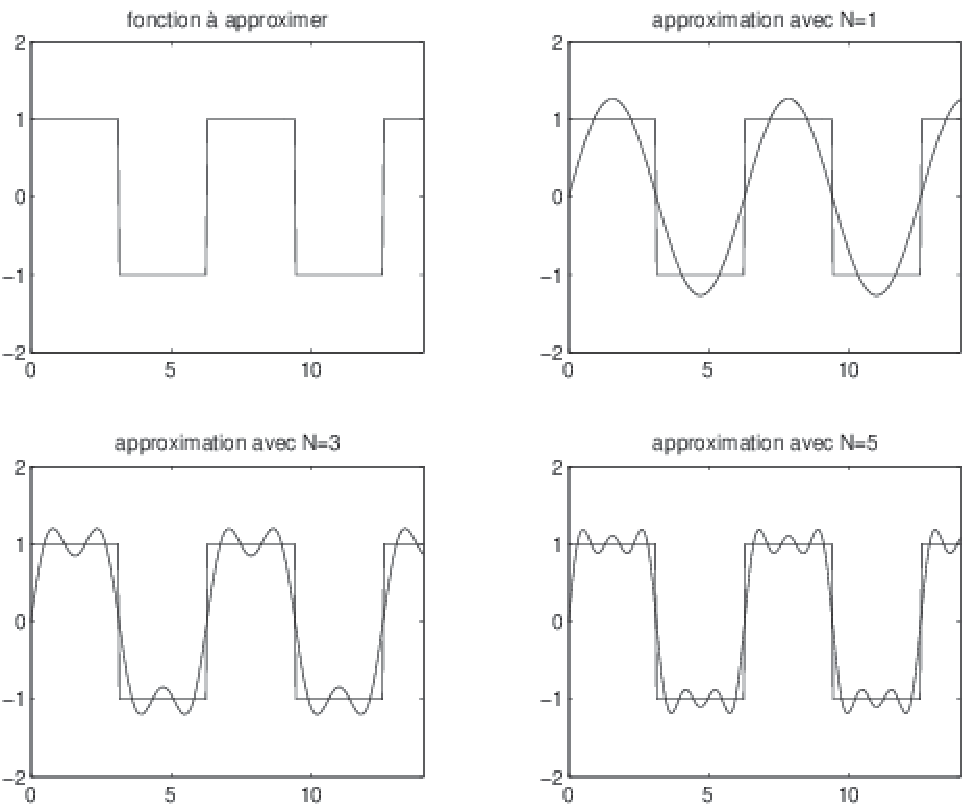
\includegraphics[scale=0.63]{reconstruction.pdf}
\caption{Transformée de Fourier d'une fonction "fenêtre". Les deux colonnes sont deux exemples ($a=1$ et $a=2$) du cas général de l'exemple \ref{ex_rectangle}. Les abscisses sont en radians.}
\end{center}
\label{fourier_transform_example}
\end{figure}

Le réel $a$ est ici un paramètre réglant la largeur de la porte, et la
transformée de Fourier de $f$ sera bien sûr fonction de $a$. Ceci
permettra de s'interroger sur la manière dont varie la transformée
quand on fait varier la largeur de la porte.  Cet exemple a une grande
importance dans les applications et mérite d'être mémorisé. %On le
retrouvera dans le chapitre sur l'analyse temps-fréquence.

\end{example}

%{\footnotesize
\begin{remark}[De la diversité des définitions (pas très important)]

Vous pourrez rencontrer, dans certaines sources d'information,
d'autres définitions de la transformée de Fourier et de la transformée
inverse, qui ne changent qu'à un facteur constant près, notamment :
\begin{equation}
F(\om)=\frac{1}{\sqrt{2\pi}}\inttotal f(t)e^{-j\om t}dt
\end{equation}
 \begin{equation}
f(t)=\frac{1}{\sqrt{2\pi}}\inttotal F(\om)e^{j\om t}d\om
\end{equation}

\end{remark}

\begin{definition}
Une fonction $f$ est dite à énergie finie (\emph{square-integrable} en anglais a le mérite de la clarté) si $\inttotal |f(t)|^2dt<\infty$. \\ On note généralement $L^2(\RR)$ l'ensemble de ces fonctions.
\end{definition}


\section{Propriétés de la transformée de Fourier}

On retrouve ici des propriétés qui étaient généralement déjà vraies et vues pour les séries de Fourier.
Pour la plupart d'entre elles, la démonstration est assez facile et un bon exercice.

\subsection{Expressions alternatives de la transformée dans des cas particuliers}

Dans les cas suivants, les simplifications obtenues n'empêchent pas
d'utiliser l'expression { standard }~\ref{reconstruction}, qui
reste parfois préférable pour la simplicité du calcul.

\begin{equation}
\text{Si $f$ est paire} \quad F(\om)=2\intpositive f(t)cos(\om t)dt
\end{equation}

 \begin{equation}
\text{Si $f$ est impaire} \quad F(\om)=-2j\intpositive f(t)sin(\om t)dt    
  \end{equation}
\subsection{Linéarité}

Soient $f$ et $g$ deux fonctions admettant une transformée de Fourier et $\lambda$ et $\mu$ deux réels. La transformée de Fourier de la combinaison linéaire est la combinaison linéaire des transformées de Fourier.
\begin{equation} \label{transfo-linearite}
\quad \BF(\lambda f+\mu g)=\lambda \BF(f)+\mu \BF(g)
\end{equation}

Un intérêt est que la transformée de Fourier d'une fonction qui n'est pas simple, mais qui peut s'exprimer comme la combinaison linéaire de fonctions élémentaires, peut être calculée par la combinaison linéaire des transformées de Fourier de ces fonctions élémentaires.

%\text{c'est-à-dire :} \quad $\BF(\lambda f+\mu g)(\omega)=\lambda \BF(f)(\omega)+\mu \BF(g)(\omega)$

\subsection{Dérivation}
Si $f'$ est la dérivée de $f$ et si elle admet une transformée de Fourier alors :
\begin{equation} \label{transfo-derivation}
  \BF(f')(\om)=j\om \BF(f)(\om)
\end{equation}


\subsection{Translation temporelle}
\label{signalretard}
Notons $f_\tau$ la fonction telle que $f_\tau(t) = f(t-\tau)$.
%
On peut montrer facilement que :
\begin{equation} \label{transfo-translation}
\BF(f_\tau)(\om)=e^{-j\om\tau} \BF(f)(\om)
\end{equation}
En particulier, remarquons que, conformément à l'intuition, la translation temporelle d'un signal ne change pas la répartition de son énergie sur l'ensemble des fréquences, mais n'affecte que la phase de la transformée :
\begin{equation}
|\BF(f_\tau)|=|\BF(f)|
\end{equation}

C'est une bonne occasion de se rappeler que le spectre fréquentiel
d'un signal, que l'on trace et que l'on interprète assez
familièrement, omet l'information de phase. Celle-ci n'en est pas pas
moins essentielle à la reconstruction du signal dans le domaine
temporel, et $F(\om)$, qui apparait dans le calcul de la transformée
inverse, est, de manière générale, une quantité complexe.

Cette propriété s'appelle parfois { théorème du retard }.  Vous
pourriez examiner et tenter d'interpréter l'effet, dans le domaine
temporel, d'une translation réalisée dans le domaine de Fourier.

\subsection{Homothétie}
Pour une réel $k>0$,
\begin{equation}
 \BF(f(kt)))=\frac{1}{k}\BF(f(\frac{t}{k}))
\end{equation}

Un cas assez simple d'application particulière, qui recoupe une situation déjà traitée, est la fonction porte de largeur quelconque.

\subsection{Égalité de Parseval}

Comme dans le cas des séries de Fourier, cette égalité établit l'égalité de l'énergie vue dans le domaine d'origine ({ temporel }) et le domaine de Fourier ({ fréquentiel }).

\begin{equation}
  \label{eq:parseval2}
  \inttotal |f(t)|^2dt=\frac{1}{2\pi}\inttotal|F(\om)|^2d\om
\end{equation}
Attention, de façon générale, il s'agit de modules sur des complexes et pas seulement de valeurs absolues apparemment superflues.

\section{Convolution, Dirac et Transformée de Fourier}

Il est utile de voir 
\begin{equation}
(f*g)(t)=\inttotal f(\tau)g(t-\tau)d\tau
\end{equation}
comme un produit scalaire entre fonctions.

La convolution est une opération qui combine deux fonctions $f$ et $g$ pour en créer une troisième, notée $f*g$. Souvent, dans les applications, $f$ est un signal et $g$ est un filtre (ou noyau)  que la convolution vient appliquer sur le signal $f$ pour l'améliorer ou en tirer une information intéressante. La convolution est aussi impliquée dans la construction de représentation de séquences ou d'images pour faire de l'apprentissage et de la reconnaissance.

Imaginons qu'un phénomène qui nous intéresse produit un signal $f(t)$ où $t$ désigne le temps, au fond de l'espace lointain. Pas de chance : comme ce signal nous vient de loin dans l'espace, ce long voyage lui fait subir des perturbations. Pour 

\begin{boxedminipage}{15cm}
\begin{definition}
Soient $f$ et $g$ deux fonctions à énergie finie.
%Soit $h(t)$ le 
Le produit de convolution entre $f$ et $g$ noté $f*g$ est défini par :

%(on note souvent $h=f*g$ ou $h(t)=(f*g)(t)$) :
\begin{equation}
(f*g)(t)=\inttotal g(\tau)f(t-\tau)d\tau
\end{equation}
\end{definition}
\end{boxedminipage}

\newcommand{\convscale}{0.52}

\begin{figure}
\begin{center}
\begin{tikzpicture}
\begin{axis}[scale=\convscale,ymin=-1.5,ymax=1.5,samples=70, xlabel={t},title={$f$}]
 \addplot[domain=0:360, blue,  ultra thick]{sin(4*x)};
\end{axis}
\end{tikzpicture}
\begin{tikzpicture}
\begin{axis}[scale=\convscale,ymin=-1.5,ymax=1.5,xlabel={$\tau$},title={$g$}]
 \addplot[domain=0:45, blue,  ultra thick]{1};
 \addplot[domain=45:360, blue,  ultra thick]{0};
\end{axis}
\end{tikzpicture}
\begin{tikzpicture}
\begin{axis}[scale=\convscale,ymin=-1.5,ymax=1.5,samples=70, xlabel={$\tau$},title={$g(\tau)f(360-\tau)$}]
  \addplot[domain=0:315, blue,  ultra thick]{0};
  \addplot[domain=315:360, blue, fill=cyan, ultra thick]{sin(4*x)};
\end{axis}
\end{tikzpicture}
\end{center}
\caption{Illustration d'une étape de la convolution. Cas particulier de $t=360$}
\end{figure}

Le produit de convolution vérifie :
\begin{eqnarray}
  f*g & =g*f & \textit{(commutativité)} \label{convolution-commut}\\
\text{~donc~} (f*g)(t) &=\inttotal f(t-\tau)g(\tau)d\tau & \\
f*(g+h) & =f*g+f*h & \textit{(distributivité)} \label{convolution-distrib}\\
(f*g)' & =f'*g=f*g' & \textit{(dérivation)} \label{convolution-derivation}
\end{eqnarray}

Il possède une propriété importante concernant la transformation de Fourier :

\begin{equation} \label{convol_transfo1}
\BF(f*g)=\BF(f).\BF(g)
\end{equation}
et dans le sens inverse :
\begin{equation}
  \BF(f.g)=\frac{1}{2\pi}\BF(f)*\BF(g)
\end{equation}

La même propriété existe d'ailleurs pour les séries de Fourier :
\begin{equation}
c_n(f*g)=c_n(f).c_n(g)
\end{equation}

Pour s'en tenir à un point de vue très pratique, la convolution donne un moyen parfois astucieux de calculer (manuellement) des transformées de Fourier de fonctions que l'on parvient à identifier comme produit de convolution de deux fonctions assez simples. 
Plus largement que le calcul de transformée, si on doit réaliser la convolution d'un signal par un filtre linéaire (par exemple filtrer un son ou une image), l'opération peut être réalisée dans le domaine de Fourier par une multiplication, ce qui permet parfois de réduire considérablement le coût (informatique) de calcul.

\begin{example}
L'exercice où on voit que la convolution d'une fonction { porte
} par elle-même donne un triangle est l'occasion d'aller creuser un
peu : le triangle est plus { lisse } que la porte (il est déjà continu,
à défaut d'être dérivable). Convoluons ce triangle par lui-même, et ce
résultat par lui-même, etc. pour voir vers quoi cela semble converger
:

\begin{center}
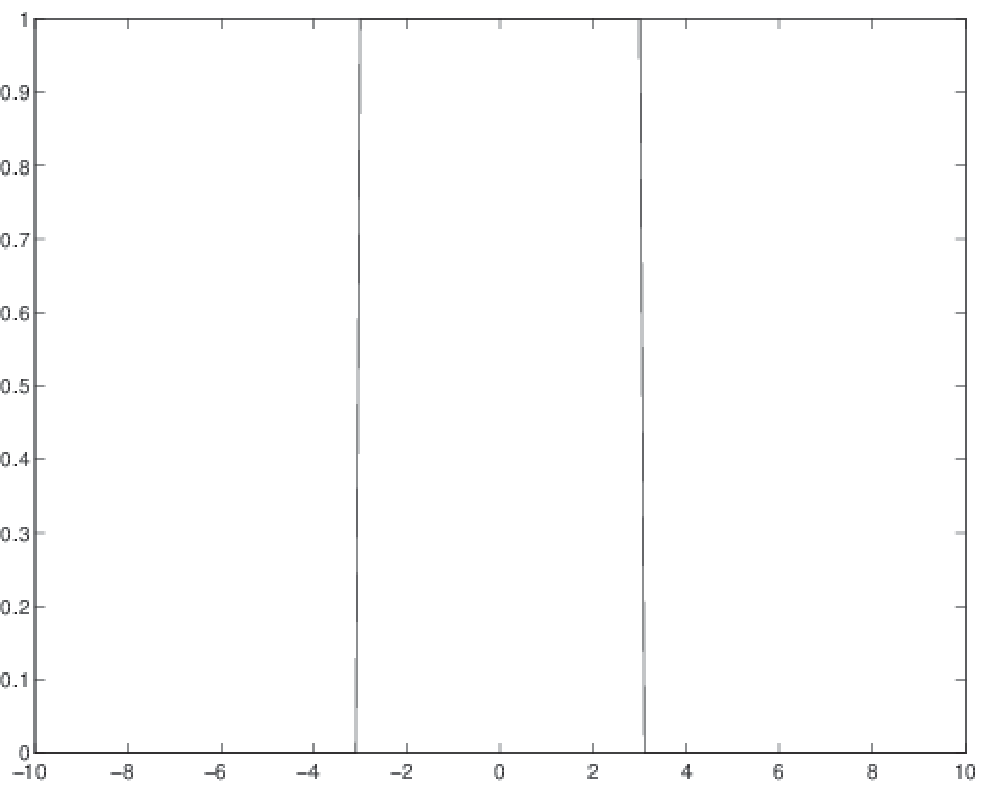
\includegraphics[scale=0.25]{convgauss1.pdf} 
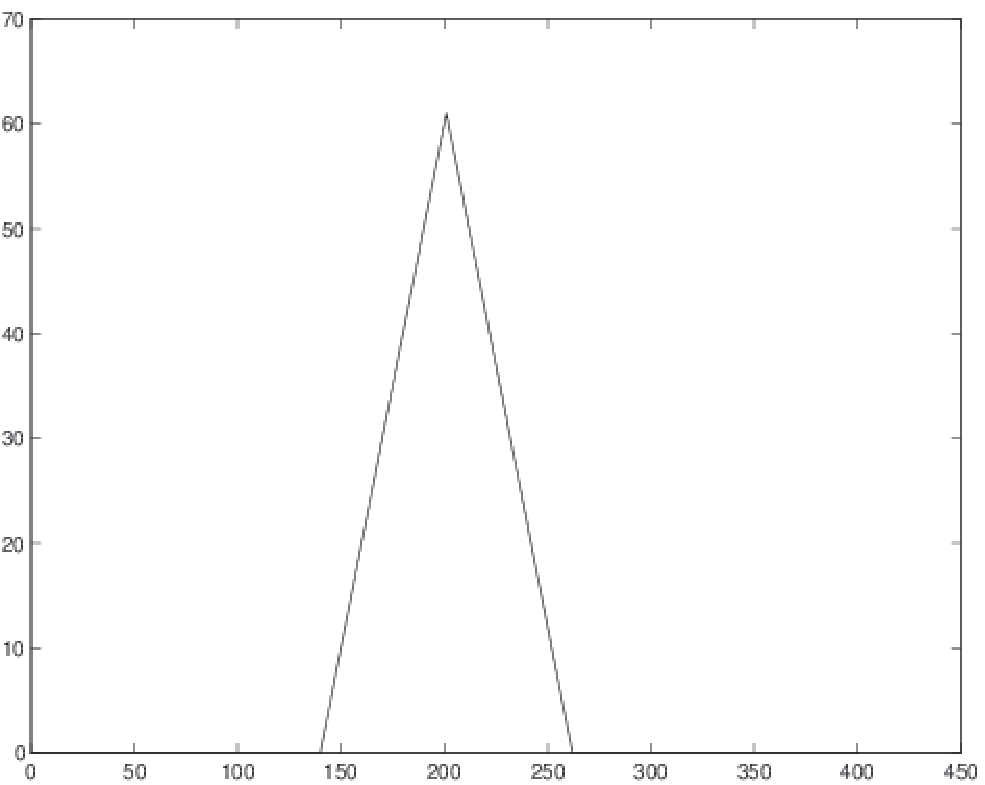
\includegraphics[scale=0.25]{convgauss2.pdf}
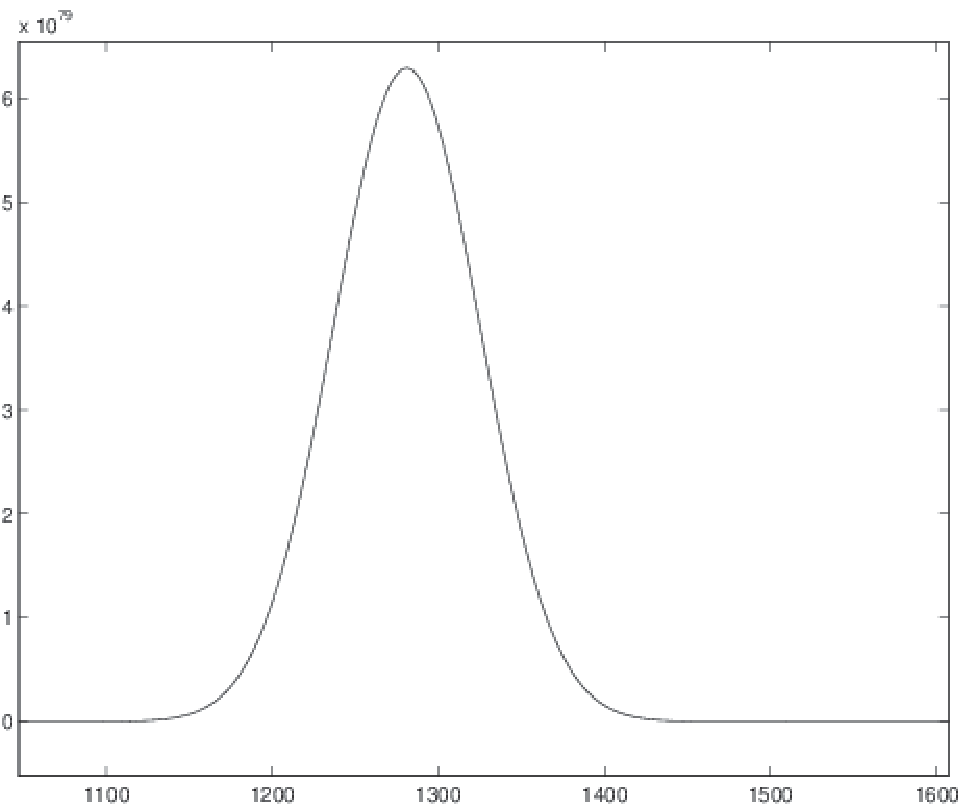
\includegraphics[scale=0.25]{convgauss3.pdf}
Fonction initiale \hspace*{1cm} Après 1 itération \hspace*{1cm} Après 6 itérations \\
\end{center}

Ce processus semble converger vers une forme gaussienne.  Un indice
supplémentaire allant dans le sens de cette supposition est que la
convolution d'une gaussienne (de moyenne $\mu_1$ et de variance
$\sigma_1^2$) par une gaussienne (de moyenne $\mu_2$ et de variance
$\sigma_2^2$) donne une gaussienne (le montrer est un bon exercice):

\begin{equation}
(\frac{e^\frac{(t-\mu_1)}{2\sigma_1^2}}{\sigma_1\sqrt{2\pi}})*
(\frac{e^\frac{(t-\mu_2)}{2\sigma_2^2}}{\sigma_2\sqrt{2\pi}})=(\frac{e^\frac{(t-(\mu_1+\mu_2))}{2(\sigma_1^2+\sigma_2^2)}}{\sqrt{2\pi(\sigma_1^2+\sigma_2^2)}})
\end{equation}

\end{example}

Au passage, une autre propriété remarquable :
\begin{equation}
  \inttotal (f*g)(t) dt=\inttotal f(t)dt \inttotal g(t)dt
\end{equation}

\subsubsection*{Illustrations}

Souvent, dans les applications de la convolution, une fonction est un
signal provenant de mesures (d'une antenne, les cours de la bourse ou
la pression atmosphérique...) et l'autre est dit { fonction noyau } (ou
simplement { noyau }), dont la forme est choisie pour modifier, analyser
ou améliorer le signal d'une façon utile.

\begin{example}
Le premier exemple (fig. \ref{fig:ex1}) montre comment on peut
approximativement { retirer le bruit } sur un signal par
convolution du signal bruité en le convoluant par une fonction
gaussienne (où on commencera à se dire { tiens, c'est simplement une
moyenne locale pondérée, un effet de lissage }).
%
\begin{figure}[h]
%
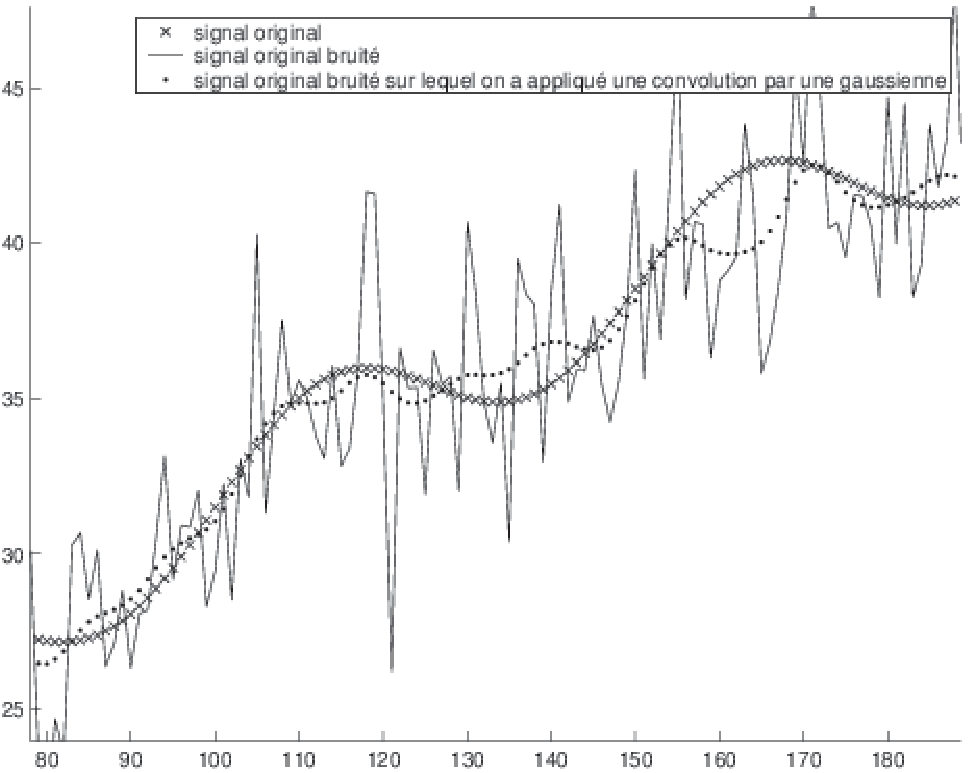
\includegraphics[scale=0.32]{con2.pdf}(a)
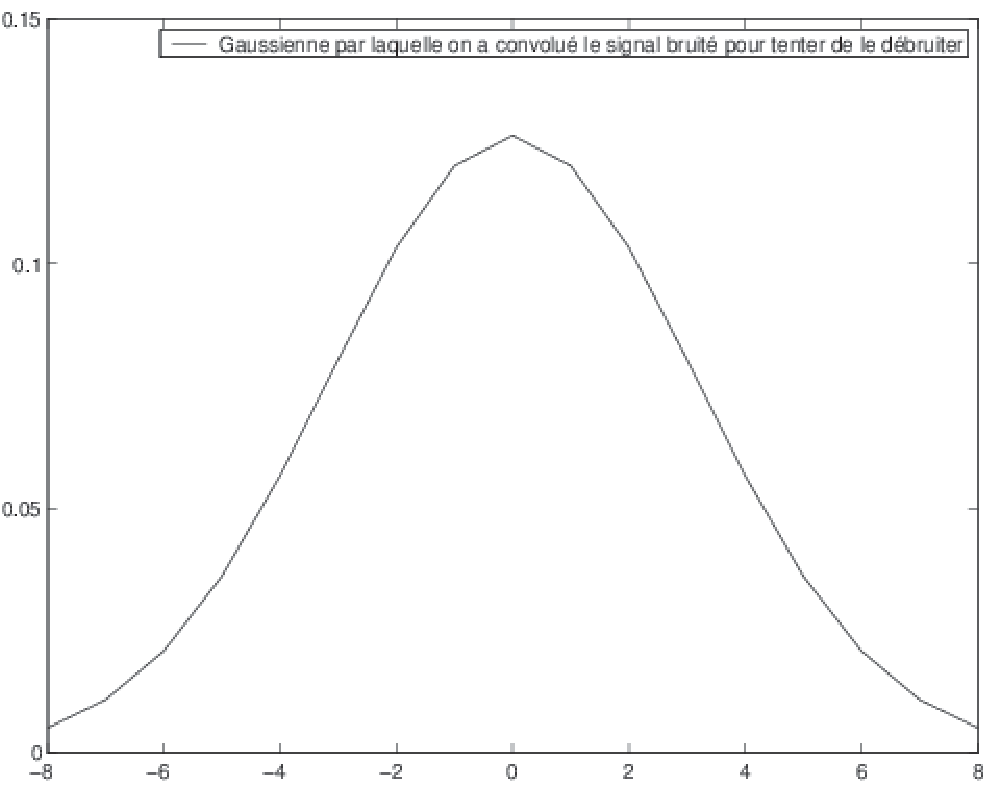
\includegraphics[scale=0.32]{con3.pdf}(b)
%
\caption{(a) Signal original : une oscillation montante, sur lequel on
a ajouté du bruit aléatoire indépendant entre instants successifs. En
convoluant ce signal bruité avec la fonction gaussienne montrée à la
figure (b), on réalise, de fait, un lissage local dans le temps,
permettant de récupérer (à peu près) le signal avant l'introduction du
bruit.}
%
\label{fig:ex1}
\end{figure}
\end{example}

\begin{example}
Le second exemple montre comment on peut détecter des discontinuités
fortes dans un signal, en convoluant le signal (on a choisi un signal
comportant des variations brusques) avec un noyau { dérivée de
gaussienne } (où on commencera à se dire { tiens, ca ressemble fort à
une sorte de calcul de dérivée }).

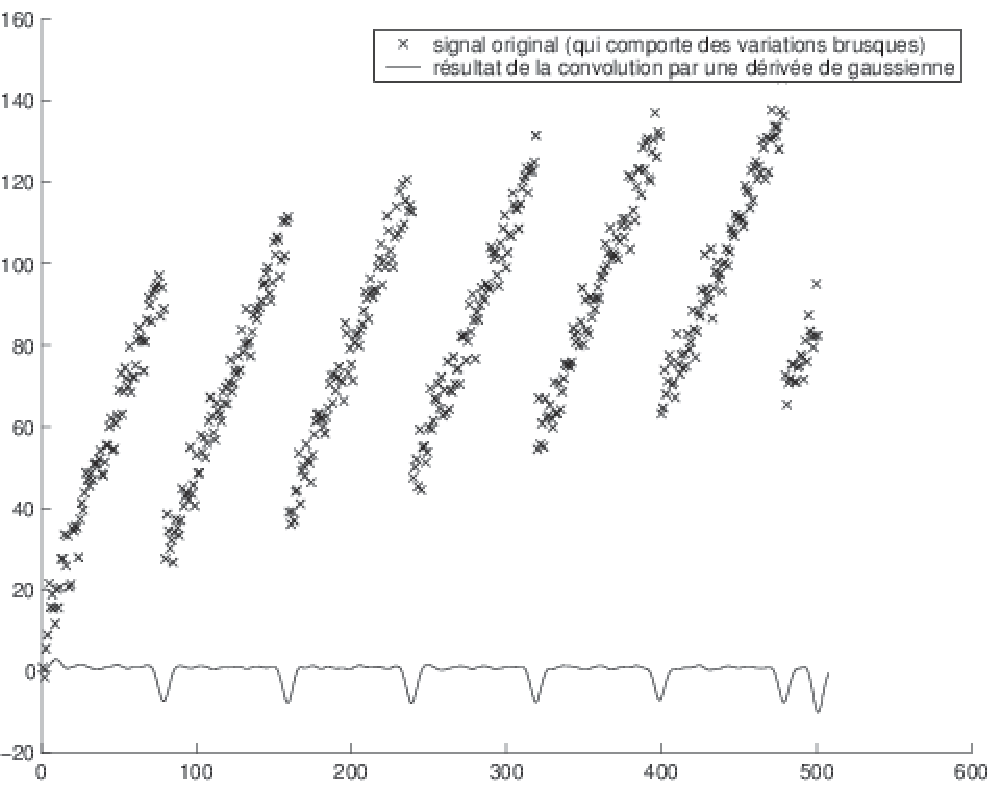
\includegraphics[scale=0.38]{con4.pdf} 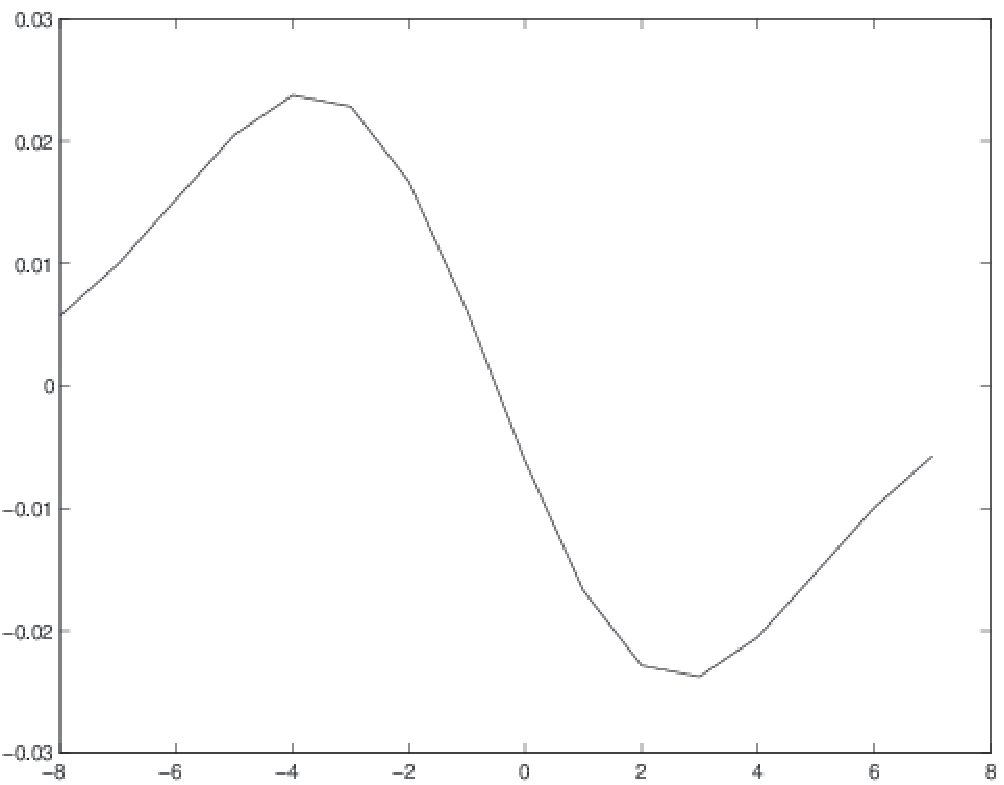
\includegraphics[scale=0.38]{con5.pdf} 
Ci-dessus à droite : fonction { dérivée de gaussienne } par laquelle on a convolué notre fonction initiale :
\end{example}

\begin{example}
En dimension 2 (cas du traitement d'image), on modélise souvent le
flou introduit par une image (par exemple en raison d'un mouvement
malheureux) comme une convolution : image floue = image nette *
operateur de flou. Remarquons au passage qu'une vision pessimiste de
notre noyau gaussien débruiteur est de dire qu'il introduit du flou
dans le signal. Une opération bien plus difficile que la convolution
mais encore plus intéressante consiste alors à trouver l'image nette à
partir de l'image floue (en particulier sans connaître l'opérateur
flouteur) : c'est une déconvolution aveugle. \\ Le même genre de
problème en dimension 1 quand un signal émis par votre téléphone
mobile veut atteindre l'antenne du réseau : il y parvient par de
multiples chemins (réflexion sur les surfaces voisines...), ce qui donne une
combinaison linéaire de diverses versions du signal émis, arrivant
avec plus ou moins de retard en fonction de la longueur de chaque
chemin. Le récepteur doit retrouver le signal d'origine, pour bien le
comprendre : voilà qui ressemble encore à notre problème de
défloutage. Une technique classique consiste à transmettre (de
l'émetteur au récepteur), de temps à autre, un signal que le
récepteur connait à l'avance : la comparaison de cette connaissance
préalable avec ce qui lui parvient lui permettra d'estimer l'opération
de { flou } causé par les chemins multiples. Il pourra utiliser
cet estimé pour déflouter la voix ou des données de l'utilisateur qui
lui parviennent les quelques secondes suivantes...
\begin{center}
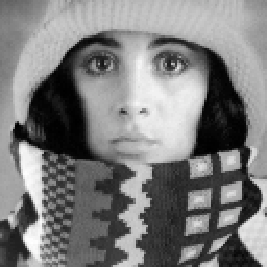
\includegraphics[scale=1]{image1.pdf} 
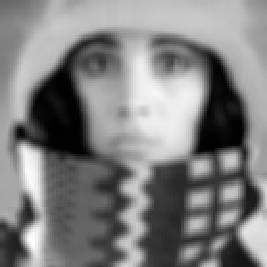
\includegraphics[scale=1]{image2.pdf}
Image originale \hspace*{2cm} Image convoluée par une gaussienne 2D \\
\end{center}
\end{example}

\subsection{Impulsion de Dirac et transformation de Fourier}
%\begin{equation*}

\begin{definition}

Considérons une fonction rectangle : 
\begin{equation}
    v(t)=
\begin{cases}
  0   & \text{si}~t \in [-\varepsilon,+\varepsilon] \\
  \frac{1}{2\varepsilon} & \text{sinon}
\end{cases}
\end{equation}
\begin{center}
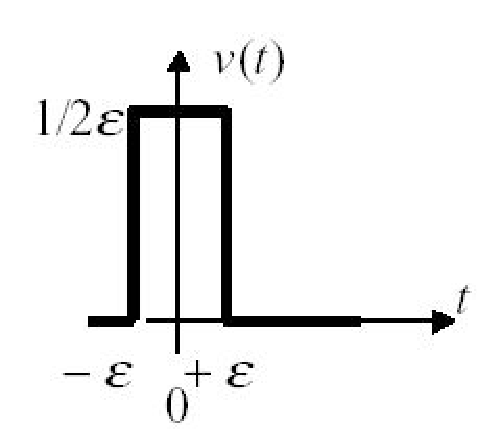
\includegraphics[scale=0.38]{dirac1.pdf} 
\end{center}

L'impulsion de Dirac est obtenue en faisant tendre $\varepsilon$ vers 0 : le rectangle est infiniment haut, infiniment étroit mais reste d'aire 1 à la limite. On aurait pu obtenir cette même limite à partir d'une fonction rectangle non nulle sur $[0,2\varepsilon]$, ou encore d'une fonction { triangle }...
où le $1$ indique l'aire et non la valeur de l'impulsion en 0 (qui est $+\infty$).
L'impulsion de Dirac est caractérisée par les propriétés suivantes :

\begin{eqnarray}
    \delta(t)=
\begin{cases}
  0   & \text{si}~t\neq0 \\
  \infty & \text{si}~t=0 
\end{cases}
\end{eqnarray}
\begin{equation}
  \inttotal \delta(t)dt~=~1
\end{equation}
\end{definition}

Le terme informel { impulsion } reste vague quant à la nature mathématique de cet objet.
Cette impulsion n'est en fait pas une \emph{fonction}, mais une \emph{distribution},
 les distributions étant une généralisation de la notion de fonction. Ces extensions sont des apports de travaux des années 1920-1950. 

L'impulsion de Dirac est notée graphiquement :
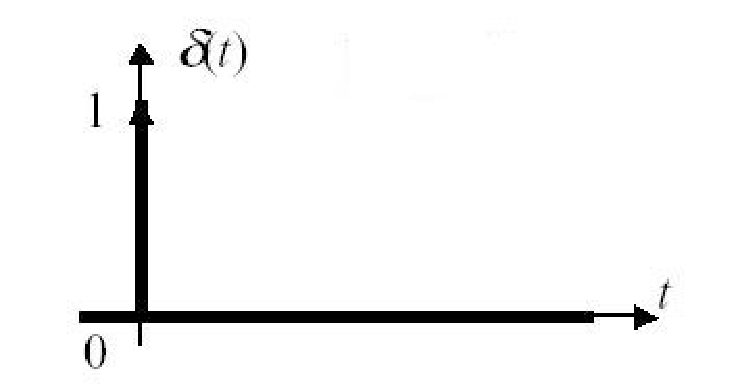
\includegraphics[scale=0.38]{dirac2.pdf} 

\begin{proposition}

\begin{equation}
 (f*\delta)(t)=\inttotal f(\tau)\delta(t-\tau)d\tau~=~f(t)
\label{proprietedirac}
\end{equation}

Autrement dit, l'impulsion de Dirac est l'élément neutre pour la convolution.
\end{proposition}

%La figure ci-dessous illustre la propriété~\ref{proprietedirac} : quand %$\varepsilon\longrightarrow~0$, le produit $f(\tau)\delta(t-\tau)$ est nul partout sauf autour %de $t=\tau$. Dans cette zone, $f(\tau)\approx f(t)$, ce qui permet de sortir $f(t)$ de %l'intégrale et de trouver le résultat~\ref{proprietedirac}.

%\begin{center}
%\input{dirac.pstex_t}
%\end{center}

Propriétés concernant l'impulsion de Dirac et la transformation de Fourier :
\begin{eqnarray}
\BF(\delta(t))~=~1 \\
\BF(1)=2\pi\delta(\om) 
\end{eqnarray}

%\end{cases}
%\end{equation*}

%Sachez aussi que l'impulsion de Dirac est la dérivée de la fonction de Heaviside (connue aussi sous le nom de fonction échelon), définie par :
%\begin{equation}
%    H(t)=
%\begin{cases}
%  1   & \text{si}~t>0 \\
%  0 & \text{sinon} 
%\end{cases}
%\end{equation}

%Remarquons qu'il y a là une extension de la notion de dérivation, puisque selon la définition usuelle, la fonction de Heaviside \footnote{La fonction paraît basique et ne méritant aucun commentaire ni même de nom particulier, jusqu'à qu'on fouille un peu de ce côté là et qu'on ouvre une boite de Pandore mathématique que l'on refermera vite ou pas (voir par ex. \emph{Analyse de Fourier et applications}, Gasquet \& Witomski pour aller plus loin.)} n'est pas dérivable en 0. Or, dans cette nouvelle dérivée, { dérivée(Heaviside)=Dirac } y compris en 0.

\subsection{Transformation de Fourier d'une fonction gaussienne}

Soit $a$ une constante strictement positive.

\begin{equation}
  \BF(e^{-at^2})=\sqrt{\frac{\pi}{a}}e^{-\frac{\om^2}{4a}}
\end{equation}


Autrement dit : la transformée de Fourier d'une gaussienne est aussi une gaussienne.

Il s'agit là d'une forme\footnote{On pourra regarder dans un second
temps la généralité de l'expression ci-dessus, pour des gaussiennes de
moyennes et variances diverses, ainsi que les constantes de
normalisation.}
%
 de fonction que l'on rencontre à chaque coin de rue,
surtout du côté des probabilités mais de manière encore plus
large. Cette propriété, qui méritera une démonstration, n'est pas
qu'esthétique - elle est par exemple exploitée dans la modulation
utilisée dans la téléphonie mobile courante.

\section{Transformée de Fourier en dimension 2}

Une application essentielle de la transformée de Fourier en dimension 2
est le traitement d'images.  La transformée existe aussi en dimension
3, utilisée pour les images { volumiques }, et également en
dimension plus élevée.

\begin{equation}
  \BF(\om_1,\om_2)=\inttotal \inttotal f(u,v)e^{-j(\om_1u+\om_2v)}~du~dv
\end{equation}
et la transformée inverse (où on omettra le cas des discontinuités) :
\begin{equation}
  f(u,v)=  \frac{1}{(2\pi)^2} \inttotal \inttotal \BF(\om_1,\om_2)e^{j(\om_1u+\om_2v)}~d\om_1~d\om_2
\end{equation}

On verra en exercice des cas où le calcul de la transformée, qui implique un calcul d'intégrale double, peut (ou pas) se formuler comme le produit de deux transformée en dimension 1.

\exercice
%
Déterminer la transformée de Fourier de la fonction suivante (fonction
{ porte } ou { impulsion rectangulaire }) :
%
\begin{equation*}
p(t) =
\begin{cases}
1 & \mbox{si } t \in ] - \frac{a}{2},\frac a 2 ]\\
0 & \mbox{sinon}
\end{cases}
\end{equation*}

\exercice
%
Démontrer les propriétés suivantes de la transformation de Fourier :
\begin{enumerate}
\item dérivation (propriété~\ref{transfo-derivation}),
\item translation (propriété~\ref{transfo-translation}),
\item linéarité (propriété~\ref{transfo-linearite}).
\end{enumerate}

\exercice Déterminer la transformée de Fourier de la fonction suivante
(fonction { triangle } ou { impulsion triangulaire }) :
%
\begin{equation*}
f(t) =
\begin{cases}
-\frac 1 a  t + 1 & \mbox{si } t \in [ 0, a ]\\
\frac 1 a  t + 1 & \mbox{si } t \in [ -a, 0 [\\
0 & \mbox{sinon}
\end{cases}
\end{equation*}


\exercice En utilisant les propriétés de la transformée de Fourier,
déterminer la transformée de Fourier de la fonction triangle (donnée
ci-dessus) en utilisant le fait qu'on peut exprimer la dérivée de la
fonction triangle en fonction de la fonction porte.


\exercice \label{convol-porte} Déterminer le produit de convolution de la fonction porte
par elle-même.

\exercice 
Démontrer les propriétés suivantes du produit de convolution :
\begin{enumerate}

\item commutativité (propriété~\ref{convolution-commut}),

\item distributivité (propriété~\ref{convolution-distrib}),

\item dérivation (propriété~\ref{convolution-derivation}).

\end{enumerate}

\exercice Démontrer la propriété~\ref{convol_transfo1} du produit de convolution par rapport à la transformation de Fourier.

\exercice Déterminer la transformée de Fourier de la fonction triangle
en utilisant les propriétés du produit de convolution et le produit
de convolution de la fonction porte par elle-même.

\exercice Déterminer la transformée de Fourier de la fonction suivante définie sur $\mathbb R^2$ :
%
\begin{equation*}
f(x,y) =
\begin{cases}
 1  & \mbox{si } -1 \leq x \leq 1 \mbox{ et } -1 \leq y \leq 1\\
0 & \mbox{sinon}
\end{cases}
\end{equation*}


\exercice Déterminer la transformée de Fourier de la fonction suivante (gaussienne) :
$$f(t) = e^{-\pi t^2}$$

%\include{temps_frequence}

\end{document} 


